\chapter{Gomulscy z Anieliny, Wólki Mińskiej, Mikanowa i~Karoliny}

% Przednia okładka podrozdziału
\includepdf{Anielina_mapa_fin.png}

\section{Anielina: 1853~r. - 2025~r.}

Wieś Anielina została założona około 1820~roku w~odległości około dwóch 
kilometrów na południe od Mińska Mazowieckiego, na terenie ówczesnego 
Królestwa Polskiego\footnote{Od 1~stycznia 1986~roku Anielina stała się 
częścią Mińska Mazowieckiego i~nie funkcjonuje już jako samodzielna 
miejscowość.}. Anielina należała na początku XIX~wieku do parafii pod 
wezwaniem Narodzenia Najświętszej Maryi Panny w~Mińsku Mazowieckim. Na 
początku swojego istnienia wieś Anielina nosiła następujące nazwy w~księgach 
metrykalnych parafii w~Mińsku Mazowieckim: \enquote{Kolonia Anielin}, 
\enquote{Anielin} oraz \enquote{Angelin}, dopiero z~czasem utrwaliła się 
obecnie stosowana nazwa tej miejscowości. Najstarsza znana wzmianka 
o~Anielinie pochodzi z~1822~roku - jest to wpis w~aktach stanu cywilnego 
gminy Mińsk Mazowiecki, z~pierwszego lipca 1822~roku, dotyczący zgonu 
Marianny Zawadzkiej córki Jana Zawadzkiego i~Apolonii z~domu Kossakowskiej 
(patrz: ryc. \ref{fig:anielina_1822}). Zmarła wówczas Marianna Zawadzka 
urodziła sie niespełna klika miesięcy wcześniej w~sąsiedniej wsi Zakole. Poza 
wspomnianą rodziną Zawadzkich\footnote{Co ciekawe Zawadzcy mieszkający we wsi 
Anielina w~latach dwudziestych XIX~wieku to przodkowie Marcina i~Marianny 
Zawadzkich, którzy przeprowadzili się na przełomie XIX~i~XX~wieku do nowo 
powstałej wówczas wsi Desna (obecnie Desno) - byli jedną z~rodzin
założycielskich tej miejscowości (udziałowcami spółki Desna) - losy rodziny
Zawadzkich spod Mińska Mazowieckiego zostaną szerzej omowione
w~\hyperref[sec:zawadzcy]{ załączniku numer III}~do niniejszej książki.},
wieś Anielina na początku XIX~wieku zamieszkiwały również między innymi takie
rodziny pochodzenia chłopskiego jak: Sikorscy, Ostrowscy, Baranowie, Michalscy,
Sadowscy czy Nalazkowie.

\begin{figure}[!ht]
    \vspace*{0.5cm}
    \centering 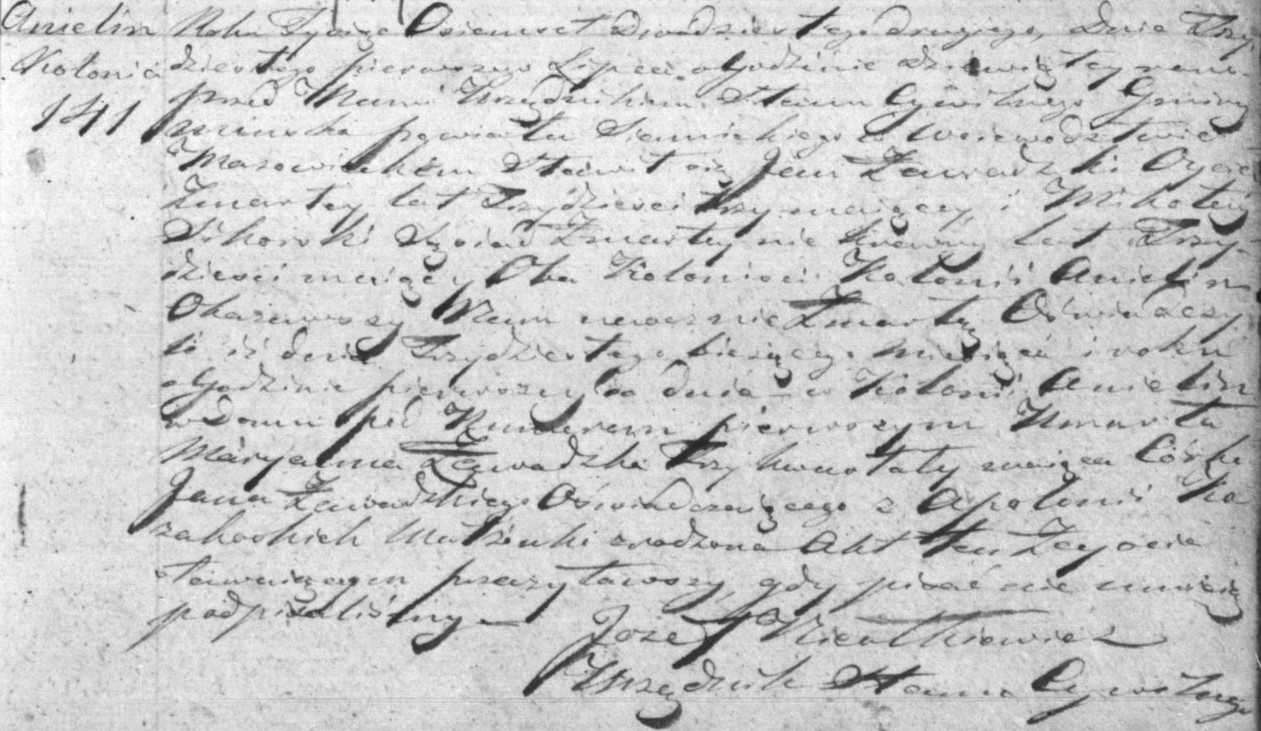
\includegraphics[width=1.0\linewidth]{
        Anielina_1822.jpg}
    \captionsetup{format=hang}
    \caption{Pierwszy znany wpis dotyczący wsi Anielina pochodzący 
    z~1822~roku z~akt stanu cywilnego gminy Mińsk Mazowiecki 
    \cite{par_minsk1}.}
    \label{fig:anielina_1822}
\end{figure}

Pierwszym dzieckiem Piotra i~Marianny Gumulskich, które urodziło się
w~Anielinie, a~zarazem ich czwartą córką, była Rozalia Gomulska. Urodziła się
ona 18~listopada 1853~roku, a~w~akcie jej chrztu jej ojciec został określony 
jako gospodarz mający 38~lat zamieszkały we wsi Angelina. Rodzicami chrzestymi 
Rozalii Gomulskiej zostali Władysław Michalski oraz Józefa Sadowska 
(patrz: ryc. \ref{fig:rgomulska_1853}).

\begin{figure}[!ht]
    \vspace*{0.5cm}
    \centering \includegraphics[width=1.0\linewidth]{
        1853_Rozalia_Gomulska_Szostak_akt_chrztu_parafia_Mińsk_Mazowiecki_wpis_260.jpg}
    \captionsetup{format=hang}
    \caption{Akt chrztu Rozalii Gomulskiej - par. Mińsk Mazowiecki 1851~rok 
    (260/1853) \cite{par_minsk2}.}
    \label{fig:rgomulska_1853}
\end{figure}

Dnia 7~października 1857~roku urodziła się najmłodsza córka Piotra i~Marianny
Gumulskich - Józefa Gomulska. W akcie jej chrztu, jej ojciec został określony 
jako \enquote{... kowal, lat czerdzieści pieć liczący, w Angelinie
zamieszkały...}. Rodzicami chrzestnymi Józefy Gomulskiej zostali Wojciech
Chłopik oraz Marianna Zawadzka (patrz: ryc. \ref{fig:jgomulska_1857}). We 
wrześniu 1859~roku we wsi Anielina na świat przyszedł Michał Gomulski, 
przedostatni syn małżeństwa Gumulskich, a~zarazem jeden z~trzech członków
rodziny Gomulskich, którzy byli założycielami wsi Desna (a~zarazem
udziałowcami spółki \enquote{Desna}) - bezpośredni potomkowie Michała 
Gomulskiego mieszkają we wsi Desno do dnia dzisiejszego, nosząc nazwisko po 
swoim przodku. W~akcie chrztu Michała jego ojciec ponownie zostal określony 
jako kowal z~Angeliny. Rodzicami chrzestnymi Michała Gomulskiego zostali Jan 
Ostrowski oraz Anna Wójcik (patrz: ryc. \ref{fig:mgomulski_1859}). 

\begin{figure}[!ht]
    \vspace*{0.5cm}
    \centering 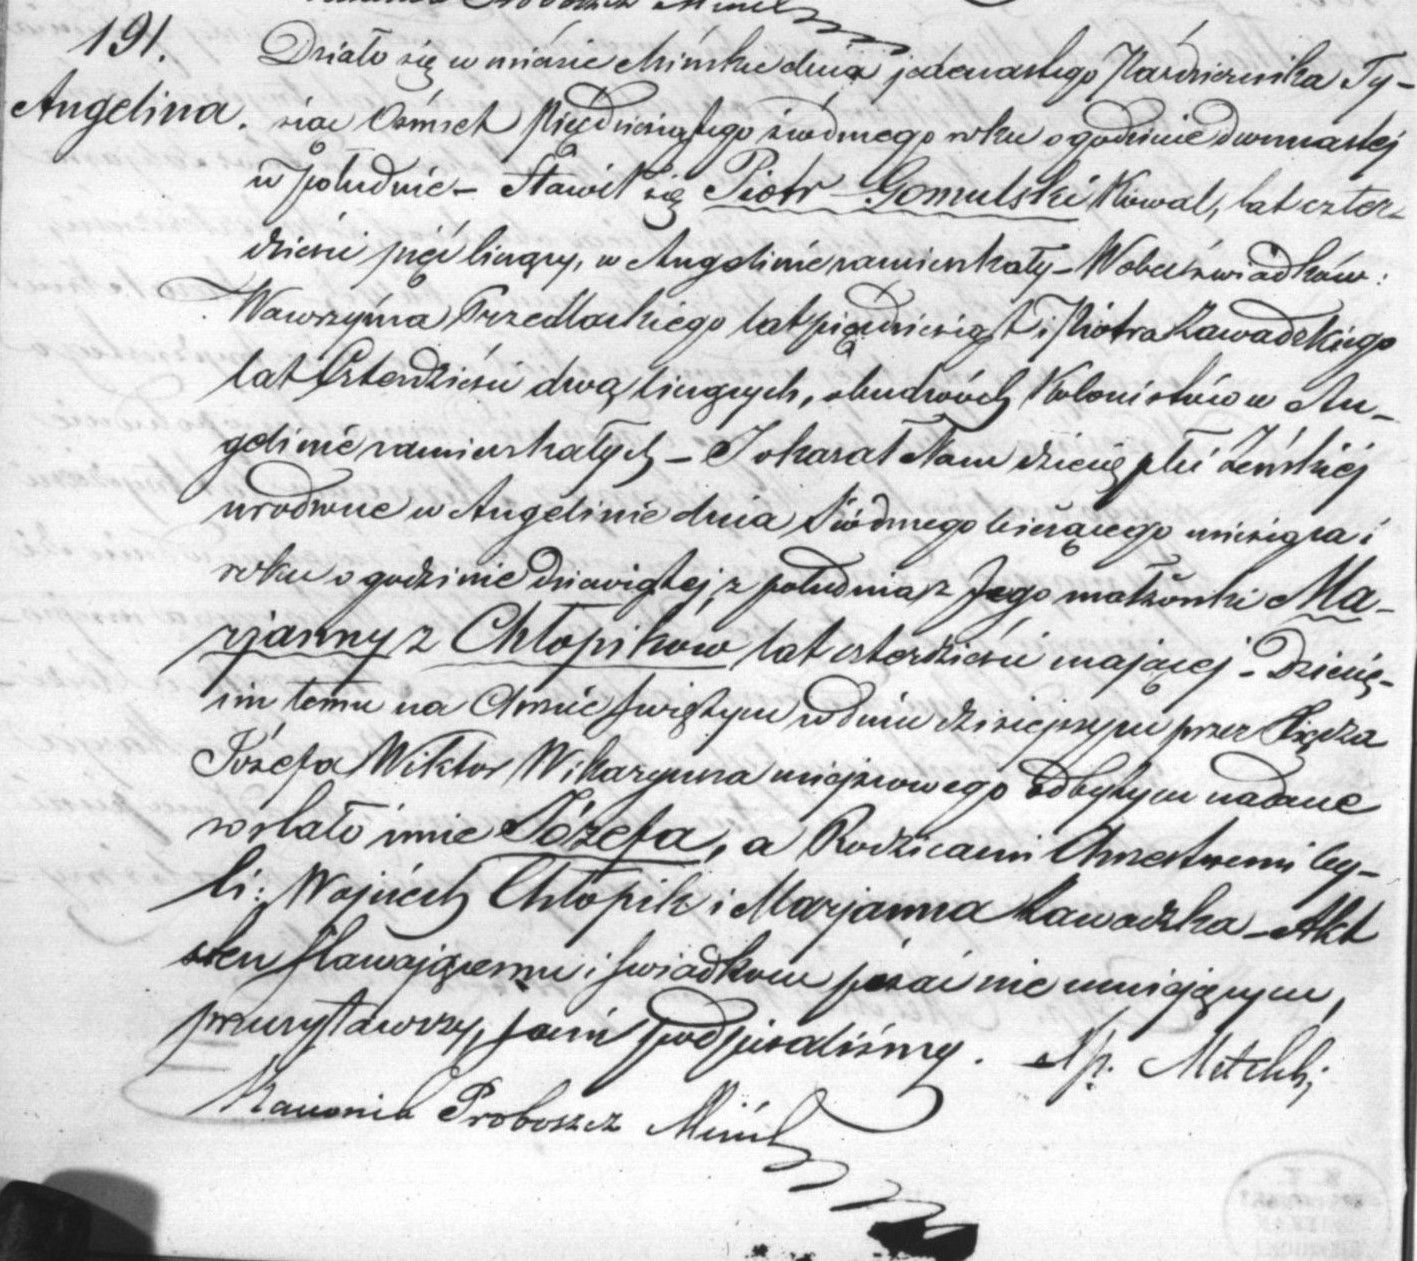
\includegraphics[width=1.0\linewidth]{
        1857_Józefa_Gomulska_akt_chrztu_parafia_Mińsk_Mazowiecki_wpis_191.jpg}
    \captionsetup{format=hang}
    \caption{Akt chrztu Józefy Gomulskiej - par. Mińsk Mazowiecki 1857~rok 
    (191/1857) \cite{par_minsk2}.}
    \label{fig:jgomulska_1857}
\end{figure}

Ostatnim dzieckiem Piotra i~Marianny Gumulskich był Stanisław Gomulski 
urodzony w~Anielinie 2~listopada 1863~roku. W~momencie jego narodzin jego 
rodzice mieli odpowiednio 48~lat (ojciec) oraz 44~lata (matka). Ojciec 
Stanisława w~akcie jego chrztu został określony jako kolonista zamieszkały 
w~Angelinie\footnote{W tamtym czasie kolonistami nazywani byli nowo przybyli 
do danej miejscowości osadnicy.}. Rodzicami chrzestnymi Stanisława Gomulskiego 
zostali Władysław Michalski oraz Katarzyna Bodzionek (patrz: ryc. 
\ref{fig:sgomulski_1863}). Stanisław, podobnie jak jego cztery lata starszy 
brat Michał, był jedynym z~założycieli wsi Desna - bezpośredni potomkowie 
Stanisława Gomulskiego mieszkają we wsi Desno do dnia dzisiejszego, ale nie 
noszą oni już nazwiska swojego przodka. Piotr i~Marianna Gumulscy mieli 
łącznie jedenaścioro dzieci, z~czego tylko sześcioro dożyło dorosłości, byli 
nimi: Jan (ur. 1836~r. - zm. 1901~r.), Grzegorz (ur. 1840~r. - zm. 1906~r.), 
Anna (ur. 1843~r. - zm. 1905~r.), Rozalia (ur. 1853~r. - zm. 1929~r.), Michał 
(ur. 1859~r. - zm. 1918~r.) i~Stanisław (ur. 1863~r. - zm. 1929~r.).

\begin{figure}[!ht]
    \vspace*{0.5cm}
    \centering 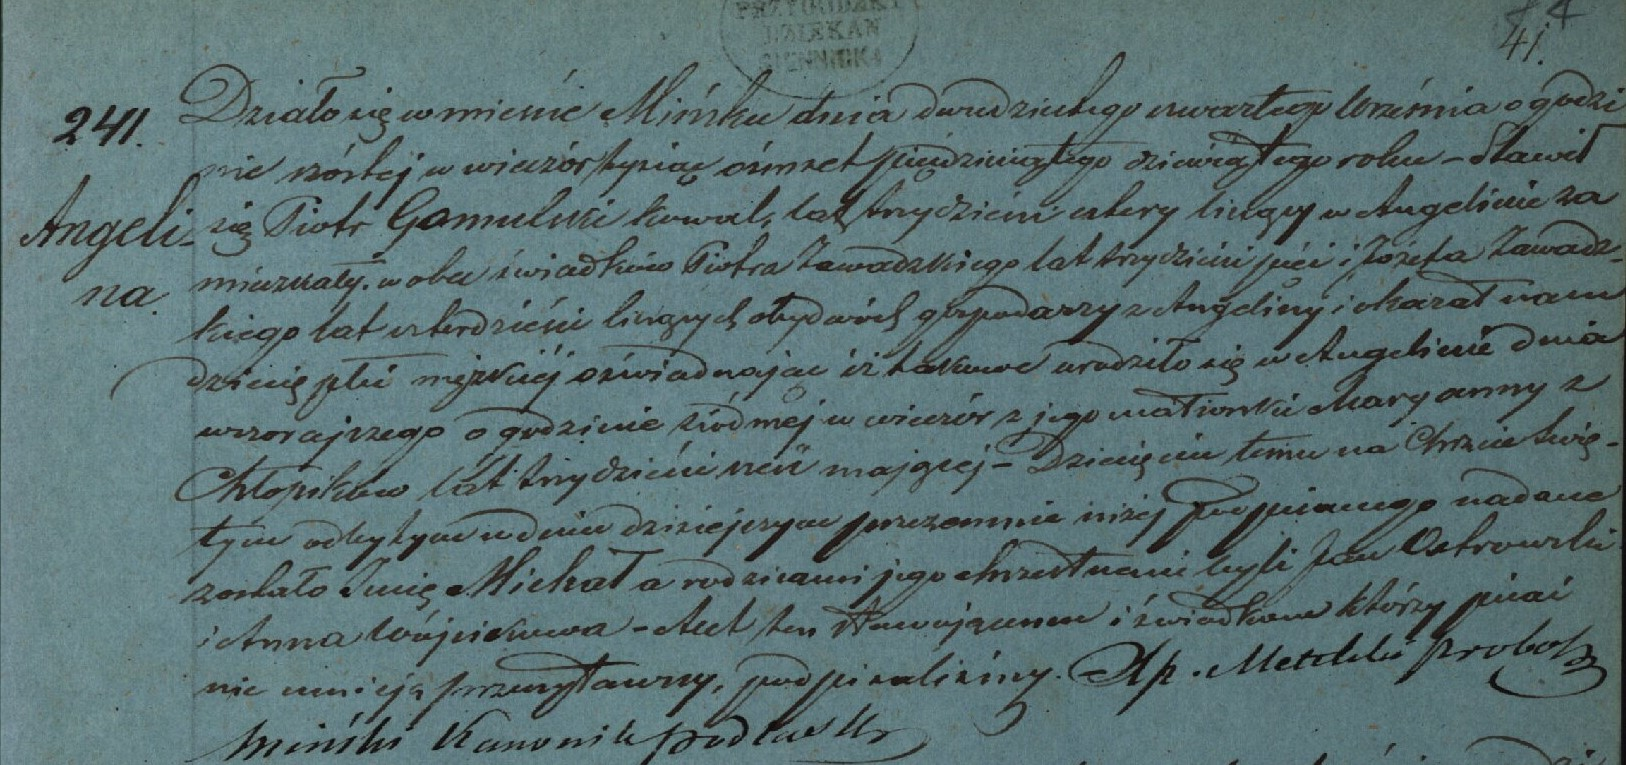
\includegraphics[width=1.0\linewidth]{
        1859_Michał_Gomulski_akt_chrztu_parafia_Mińsk_Mazowiecki_wpis_241.jpg}
    \captionsetup{format=hang}
    \caption{Akt chrztu Michała Gomulskiego - par. Mińsk Mazowiecki 1859~rok 
    (241/1859) \cite{par_minsk2}.}
    \label{fig:mgomulski_1859}
\end{figure}

\begin{figure}[!ht]
    \vspace*{0.5cm}
    \centering 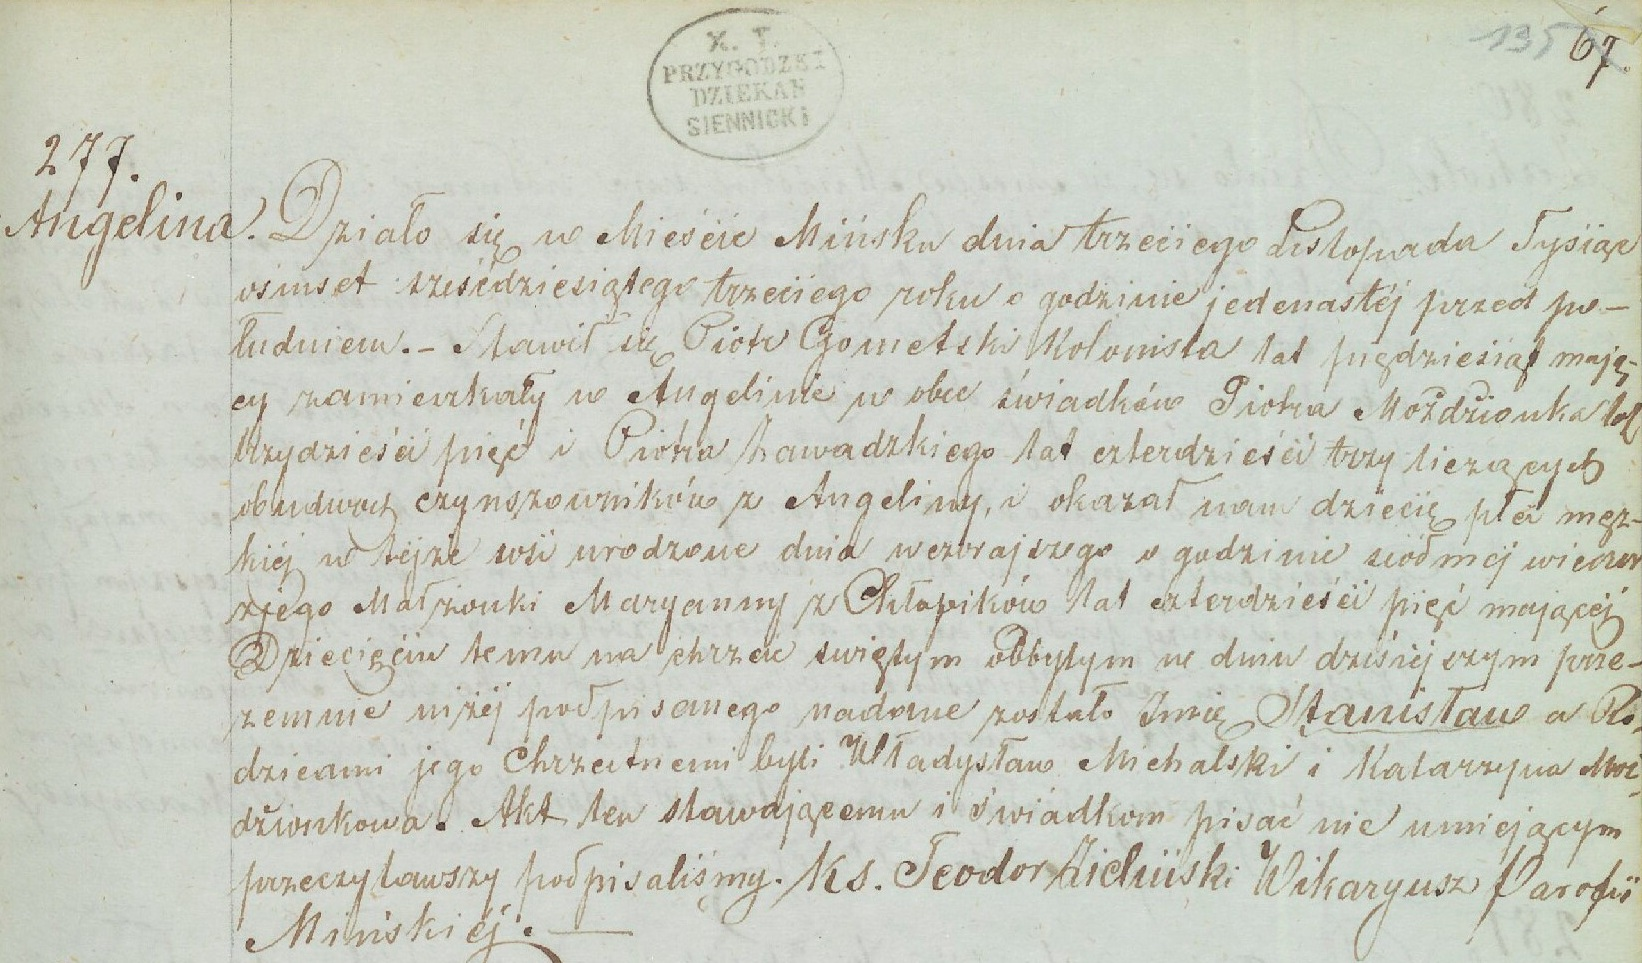
\includegraphics[width=1.0\linewidth]{
        1863_Stanisław_Gomulski_akt_chrztu_parafia_Mińsk_Mazowiecki_wpis_277.jpg}
    \captionsetup{format=hang}
    \caption{Akt chrztu Stanisława Gomulskiego - par. Mińsk Mazowiecki 
    1863~rok (277/1863) \cite{par_minsk2}.}
    \label{fig:sgomulski_1863}
\end{figure}

Piotr Franciszek Gumulski ostanie 17~lat swojego życia przeżył we wsi Anielina
 - zmarł 8~lutego 1870~roku w~wieku 55 lat (patrz: ryc.
 \ref{fig:pfgomulski_1870}\footnote{Akt zgonu Piotra Franciszka Gumulskiego 
 został sporządzony w~języku rosyjskim, gdyż począwszy od 1868~roku w~wyniku 
represji carskich po powstaniu styczniowym, wszystkie kościelne akta 
metrykalne w~Królestwie Polskim musiały być prowadzone w~języku rosyjskim - 
represje te były utrzymywane aż do 1915~roku.}). 

\begin{figure}[!ht]
    \vspace*{0.5cm}
    \centering \includegraphics[width=1.0\linewidth]{
        1870_Piotr_Franciszek_Gumulski_akt_zgonu_parafia_Mińsk_Mazowiecki_wpis_51.jpg}
    \captionsetup{format=hang}
    \caption{Akt zgonu Piotra Franciszka Gumulskiego - par. Mińsk Mazowiecki 
    1870~rok (51/1870) \cite{par_minsk2}.}
    \label{fig:pfgomulski_1870}
\end{figure}

\begin{figure}[!ht]
    \vspace*{0.5cm}
    \centering 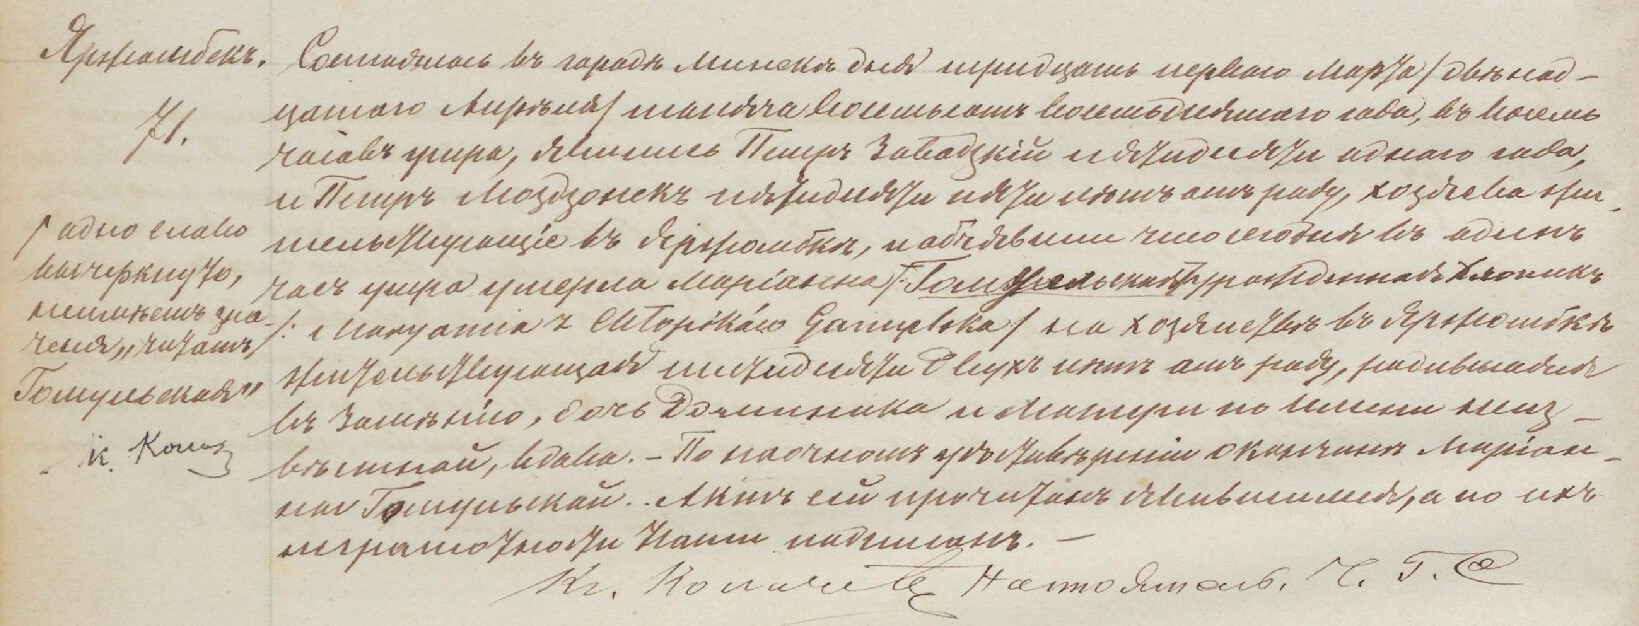
\includegraphics[width=1.0\linewidth]{
        1880_Marianna_Gumulska_Chłopik_akt_zgonu_parafia_Mińsk_Mazowiecki_wpis_71.jpg}
    \captionsetup{format=hang}
    \caption{Akt zgonu Marianny Gumulskiej - par. Mińsk Mazowiecki 
    1880~rok (71/1880) \cite{par_minsk2}.}
    \label{fig:mgomulska_1880}
\end{figure}

Marianna Gumulska (z~domu Chłopik) zmarła 10~lat po swoim mężu - 12~kwietnia 
1880~roku, dożywając wieku 61~lat. W~akcie jej zgonu wskazano, iż 
zmarła ona we wsi Jarząbek, czyli pobliskiej w~stosunku do Anieliny wsi, do 
której Marianna prawdopodobnie przeprowadziła się  ze swoim szwagrem oraz jego
 rodziną (patrz: ryc. \ref{fig:mgomulska_1880}).

\begin{figure}[!ht]
    \vspace*{0.5cm}
    \centering 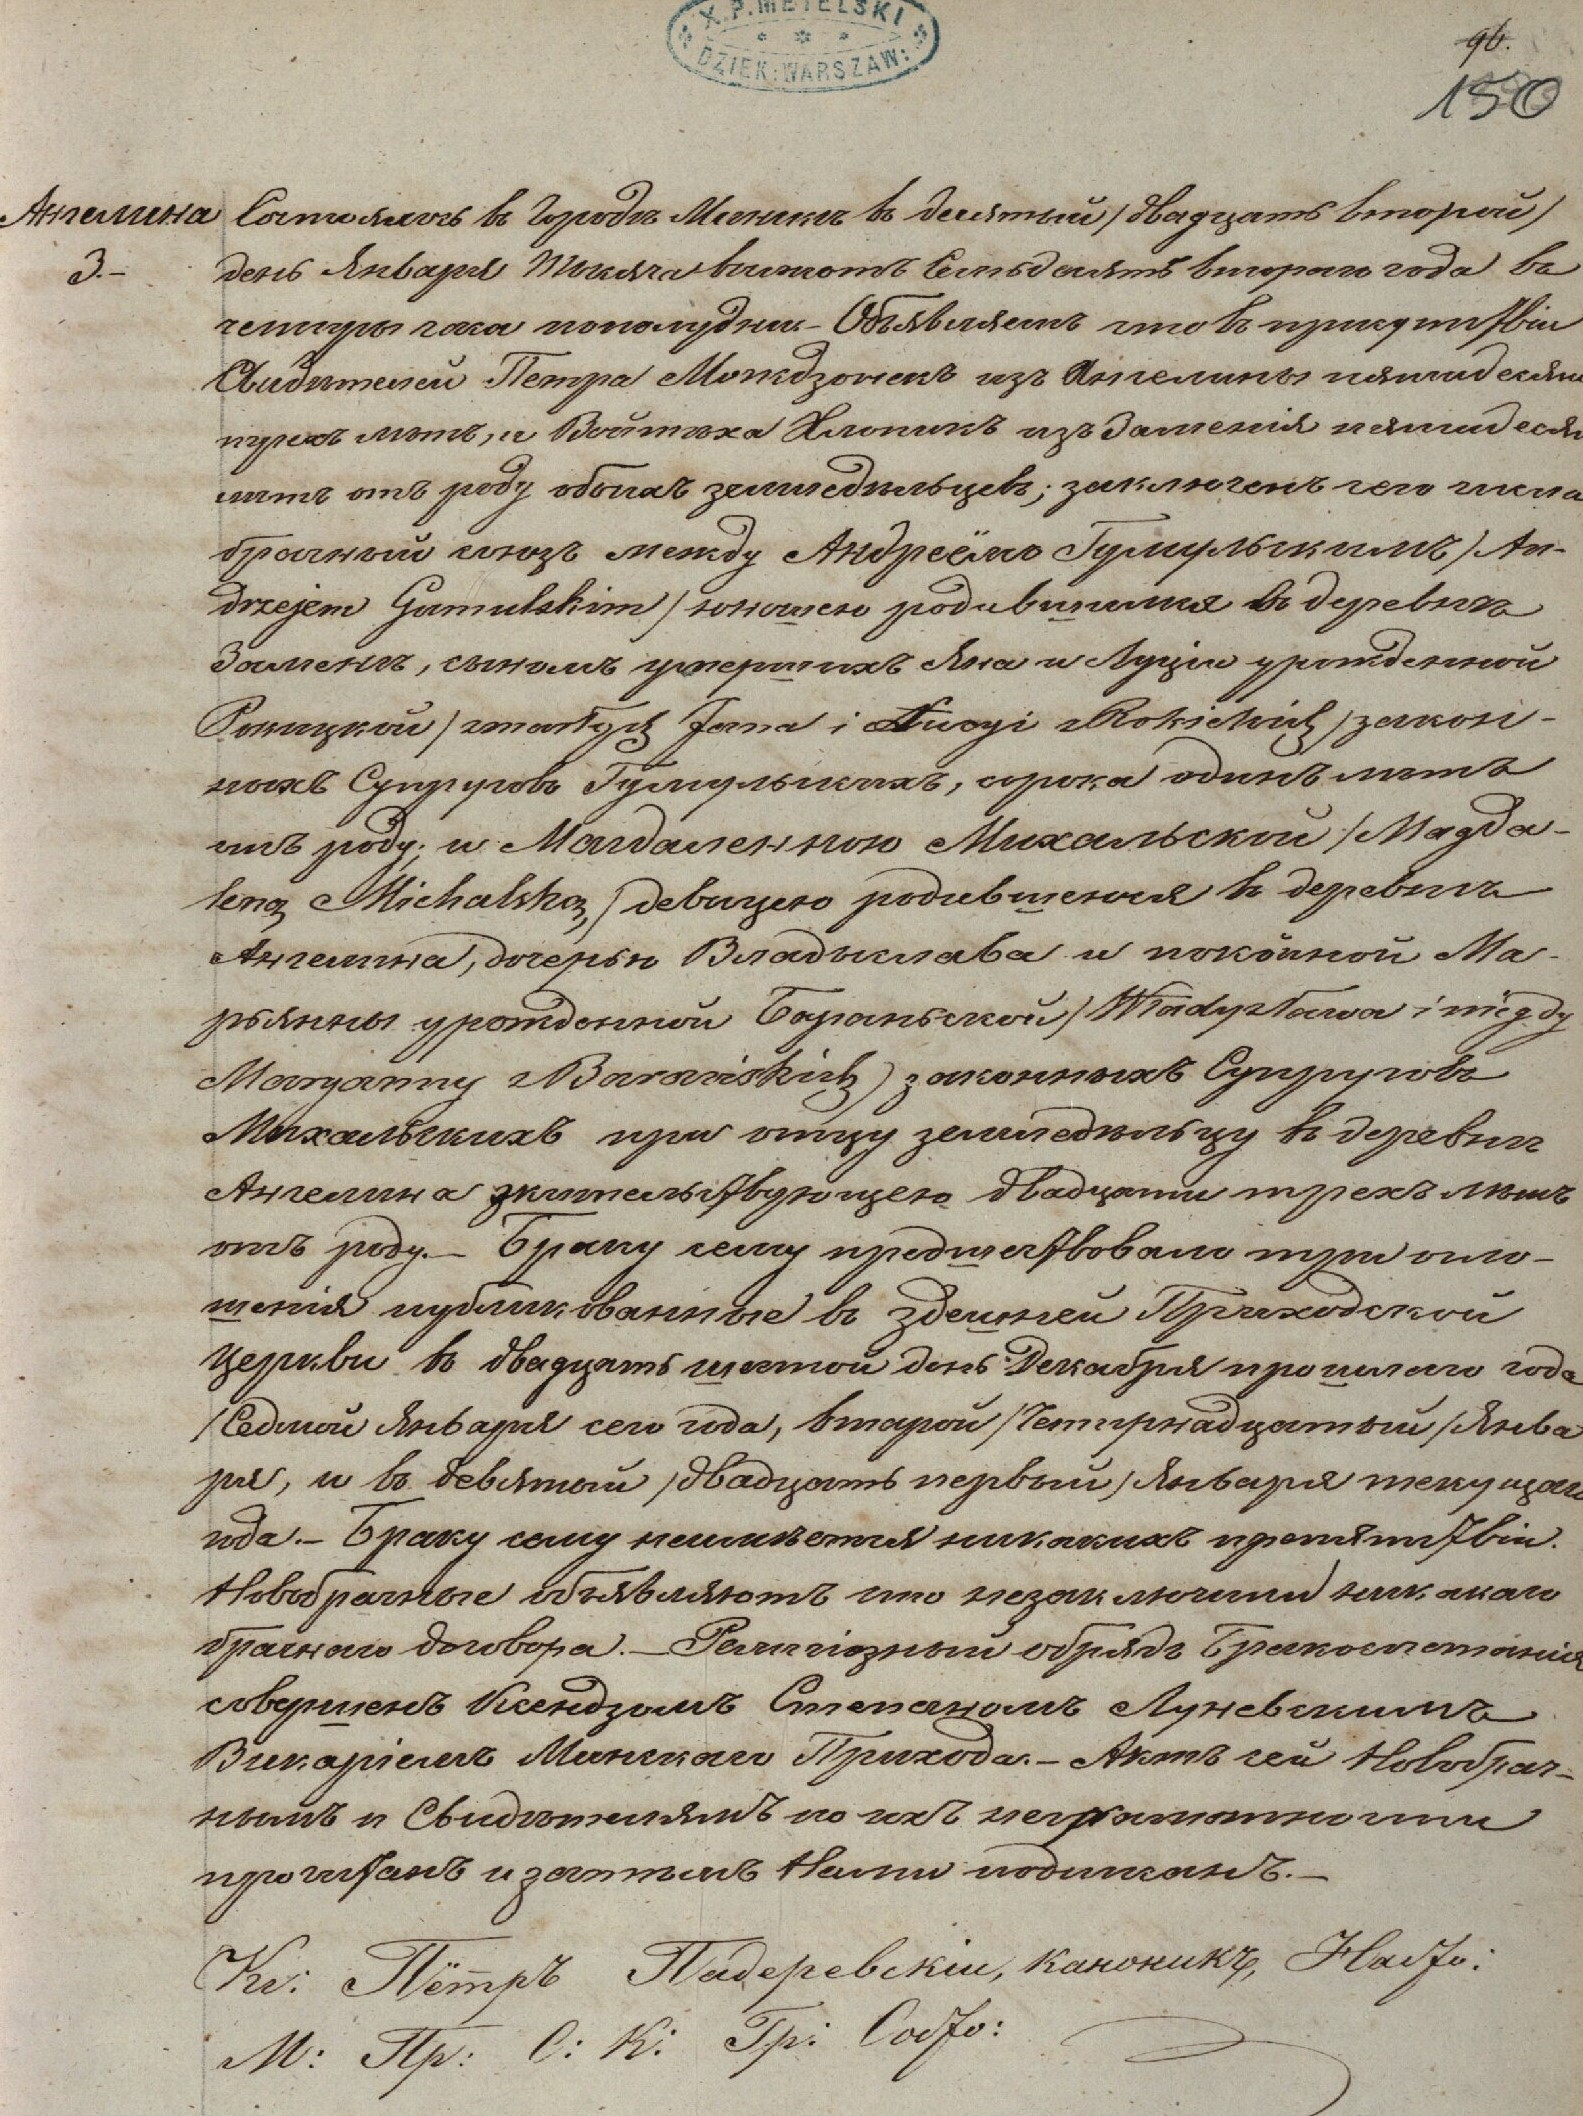
\includegraphics[width=0.92\linewidth]{
        1872_Andrzej_Gomulski_Magdalena_Michalska_akt_ślubu_parafia_Mińsk_Mazowiecki_wpis_3.jpg}
    \captionsetup{format=hang}
    \caption{Akt ślubu Andrzeja Gumulskiego i~Magdaleny Michalskiej - par. 
    Mińsk Mazowiecki 1872~rok (3/1872) \cite{par_minsk2}.}
    \label{fig:agumulski_1872}
\end{figure}

Około 1872~roku, dwa lata po śmierci Piotra Gumulskiego, do Anieliny 
przeprowadził się jego młodszy brat Andrzej. Powodem jego przeprowadzki do 
Anielny był prawdopodobnie ślub, który wziął z~lokalną dziewczyną, Magdaleną 
Michalską, 22~stycznia 1872~roku w~Mińsku Mazowieckim. Andrzej Gumulski miał 
wówczas blisko 42~lata, a~jego przyszła żona ledwo ukończyła 23 lata (patrz: 
ryc. \ref{fig:agumulski_1872}). 

  \begin{figure}[!ht]
    \vspace*{0.5cm}
    \centering \includegraphics[width=1.0\linewidth]{
        1875_Feliks_Gomulski_akt_chrztu_parafia_Mińsk_Mazowiecki_wpis_126.jpg}
    \captionsetup{format=hang}
    \caption{Akt chrztu Feliksa Gomulskiego - par. Mińsk Mazowiecki 
    1875~rok (126/1875) \cite{par_minsk2}.}
    \label{fig:fgomulski_1875}
\end{figure}

Andrzej Gumulski wraz ze swoją żoną Magdaleną dochowali się trójki dzieci, 
z~czego dwójka najstarszych urodziła się w~Anielinie, a trzecie z~nich 
urodziło się we wsi Jarząbek: 

\begin{itemize}
    \item Feliks Gomulski (ur. 1875~r. - zm. 1941~r.) - patrz: ryc. 
    \ref{fig:fgomulski_1875},
    \item Antonina Gomulska (ur. 1878~r. - zm. 1955~r.) - patrz: ryc. 
    \ref{fig:agomulska_1878},
    \item Józefę (ur. 1882~r. - zm. 1884~r.)  - patrz: ryc. 
    \ref{fig:lgomulska_1882} oraz ryc. \ref{fig:lgomulska_1884}.
  \end{itemize}

Wygląda więc na to, że Andrzej Gumulski wraz z~żoną, dziećmi oraz 
bratową Marianną przeprowadzili się do Jarząbka około 1880~roku, jednak po 
1884~roku wrócili do Anieliny, bo tam zmarł zarówno Andrzej - w~1887~roku 
(patrz: ryc. \ref{fig:agomulski_1887}), jak i jego żona Magdalena - 
w~1904~roku.

\begin{figure}[!ht]
    \vspace*{0.5cm}
    \centering 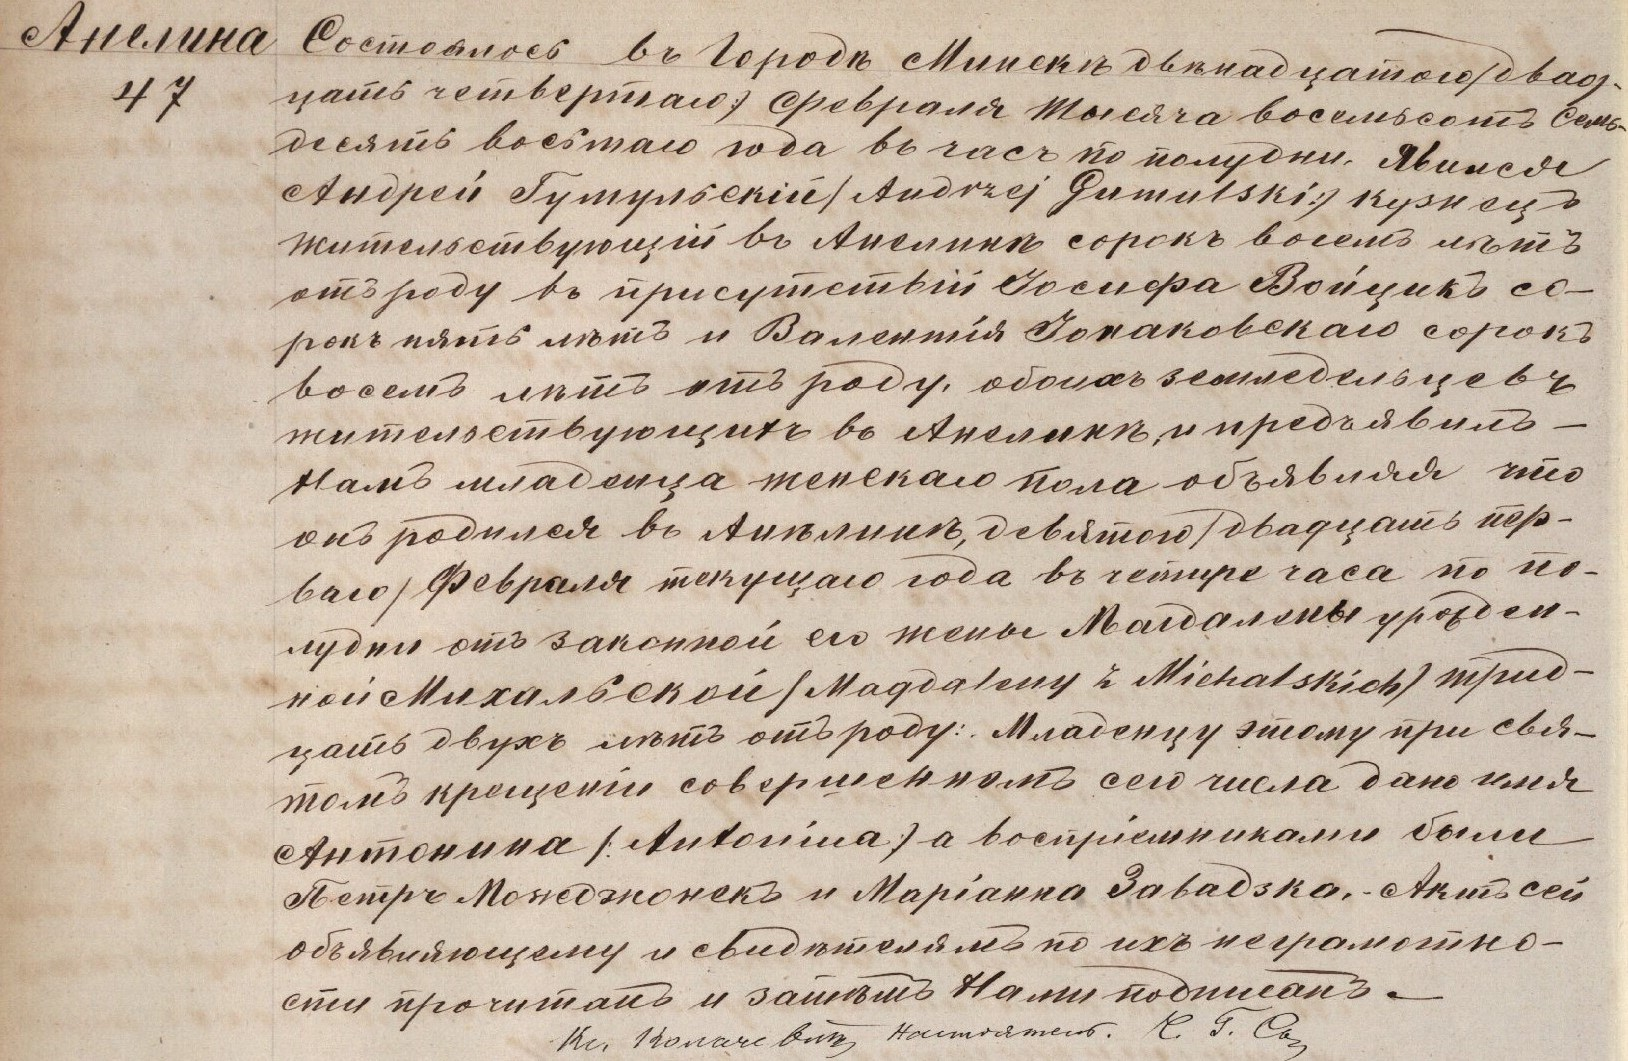
\includegraphics[width=0.99\linewidth]{
        1878_Antonina_Gomulska_Araźna_akt_chrztu_parafia_Mińsk_Mazowiecki_wpis_47.jpg}
    \captionsetup{format=hang}
    \caption{Akt chrztu Antoniny Gomulskiej - par. Mińsk Mazowiecki 
    1878~rok (47/1878) \cite{par_minsk2}.}
    \label{fig:agomulska_1878}
\end{figure}

\begin{figure}[!ht]
    \vspace*{0.5cm}
    \centering \includegraphics[width=0.99\linewidth]{
        1882_Ludwika_Gomulska_akt_chrztu_parafia_Mińsk_Mazowiecki_wpis_167.jpg}
    \captionsetup{format=hang}
    \caption{Akt chrztu Ludwiki Gomulskiej - par. Mińsk Mazowiecki 
    1882~rok (167/1882) \cite{par_minsk2}.}
    \label{fig:lgomulska_1882}
\end{figure}

\begin{figure}[!ht]
    \vspace*{0.5cm}
    \centering \includegraphics[width=0.93\linewidth]{
        1884_Ludwika_Gomulska_akt_zgonu_parafia_Mińsk_Mazowiecki_wpis_70.jpg}
    \captionsetup{format=hang}
    \caption{Akt zgonu Ludwiki Gomulskiej - par. Mińsk Mazowiecki 
    1884~rok (70/1884) \cite{par_minsk2}.}
    \label{fig:lgomulska_1884}
\end{figure}

\begin{figure}[!ht]
    \vspace*{0.5cm}
    \centering \includegraphics[width=0.93\linewidth]{
        1887_Andrzej_Gomulski_akt_zgonu_parafia_Mińsk_Mazowiecki_wpis_13.jpg}
    \captionsetup{format=hang}
    \caption{Akt zgonu Andrzeja Gumulskiego - par. Mińsk Mazowiecki 
    1887~rok (13/1887) \cite{par_minsk2}.}
    \label{fig:agomulski_1887}
\end{figure}

Z trójki dzieci Andrzeja i~Magdaleny Gumulskich tylko dwójka dożyła wieku 
dorosłego - Feliks Gomulski ożenił się w~1909~roku w~Pęcicach pod Pruszkowem 
z~Małgorzatą Makowską pochodzącą ze Słomina (patrz: ryc. 
\ref{fig:fgomulski_1909}) a~Antonina Gomulska w~1896~roku wyszła za mąż 
w~Mińsku Mazowieckim za Michała Araźnego pochodzącego ze wsi Olesin, 
znajdującej się koło Dębego Wielkiego.

\begin{figure}[!ht]
    \vspace*{0.5cm}
    \centering 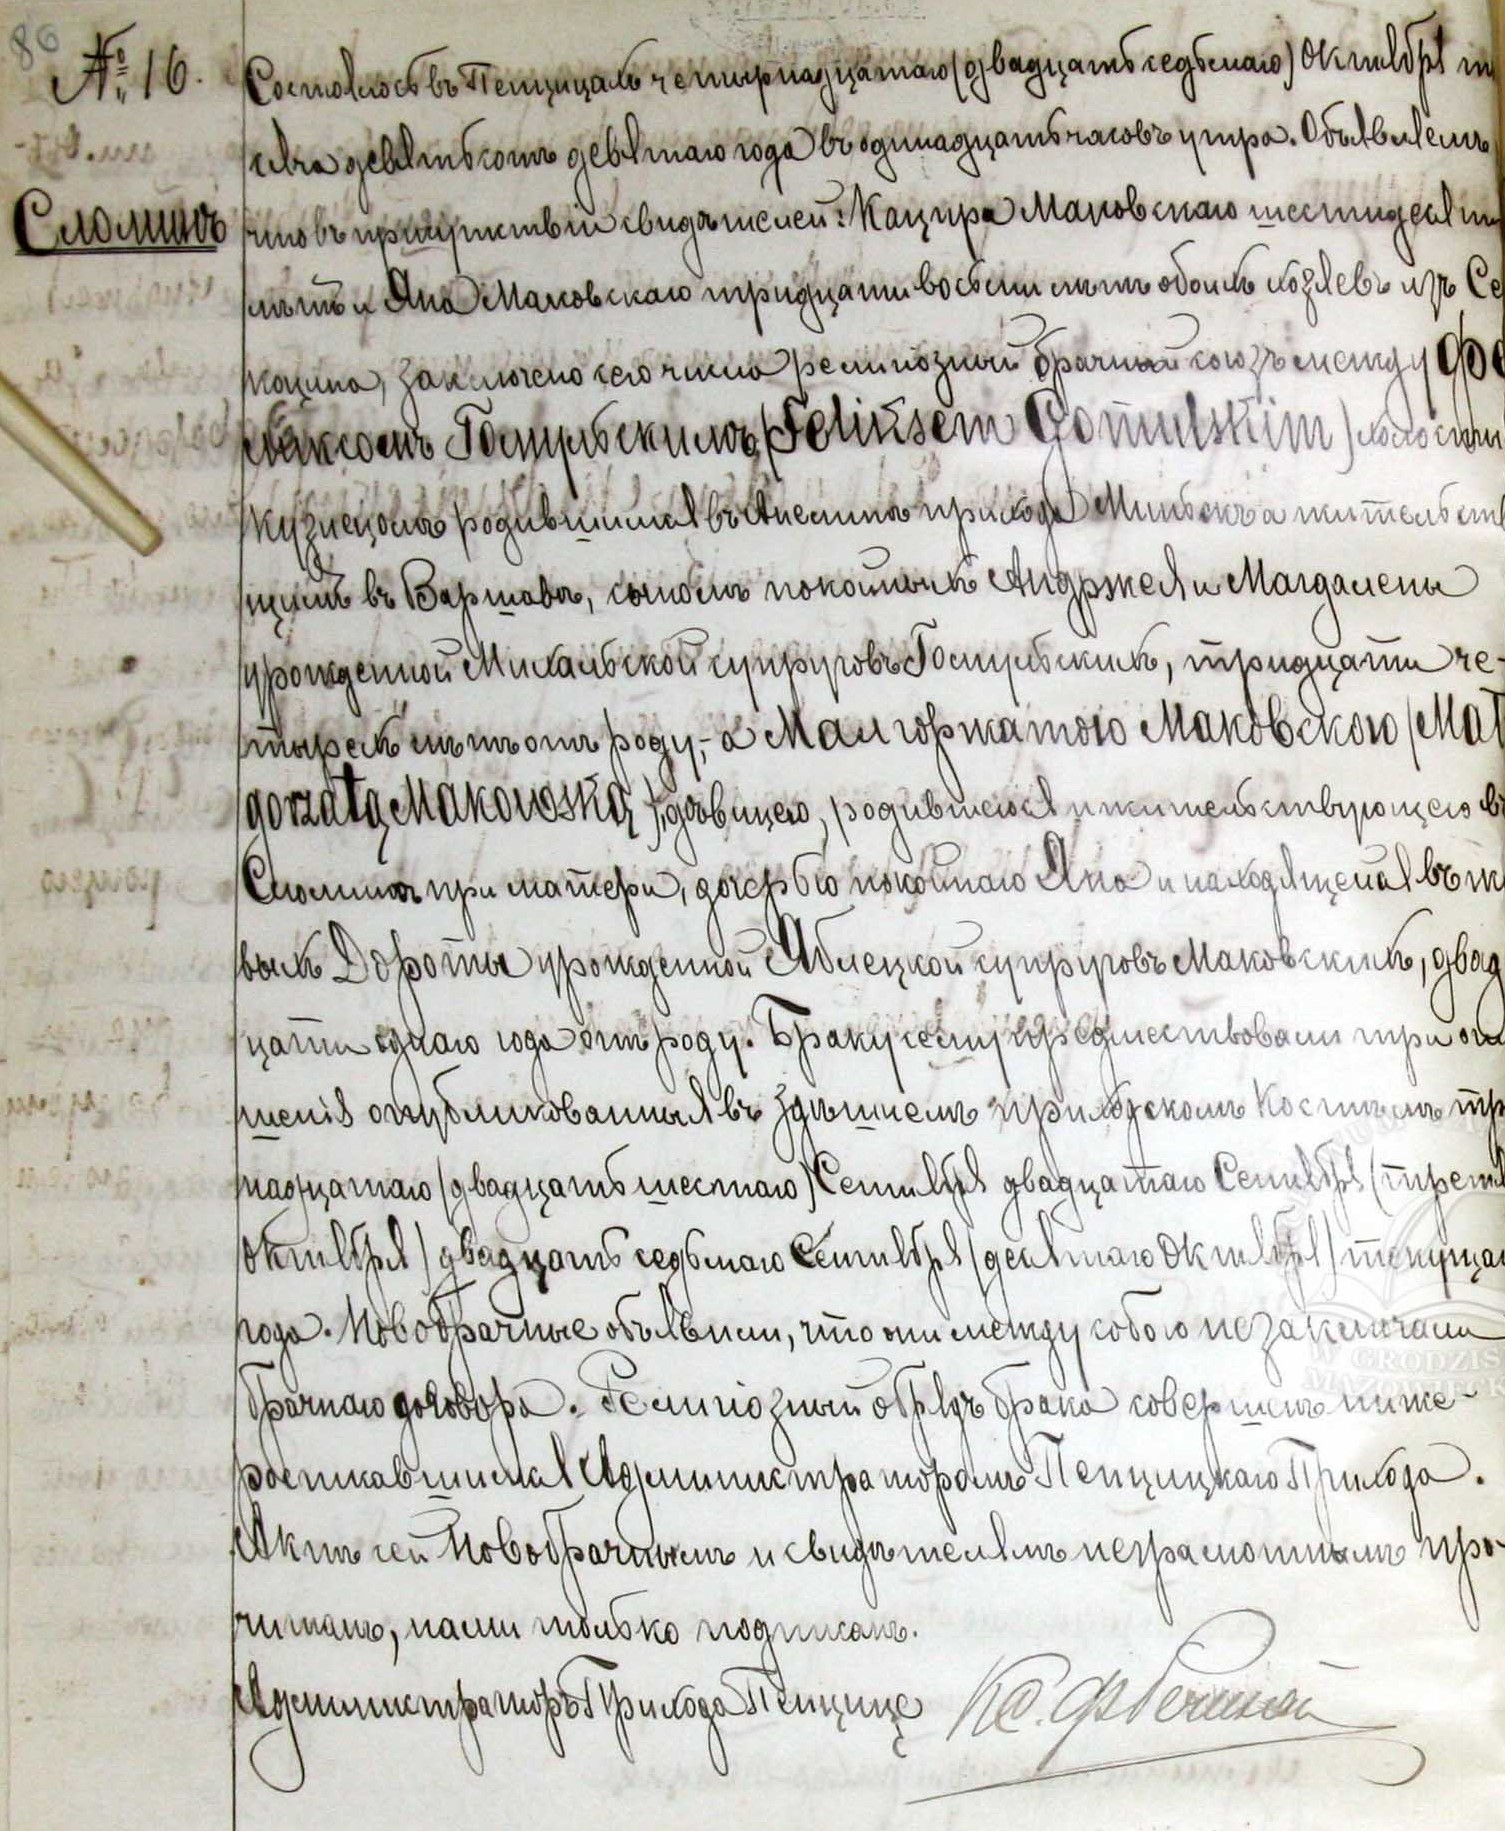
\includegraphics[width=1.0\linewidth]{
        1909_Feliks_Gomulski_Małgorzata_Makowska_akt_ślubu_parafia_Pęcice_wpis_16.jpg}
    \captionsetup{format=hang}
    \caption{Akt ślubu Feliksa Gomulskiego oraz Małgorzaty Makowskiej - par. 
    Pęcice 1909~rok (16/1909) \cite{par_pecice}.}
    \label{fig:fgomulski_1909}
\end{figure}

\begin{figure}[!ht]
    \vspace*{0.5cm}
    \centering \includegraphics[width=0.8\linewidth]{
        1910_Henryk_Gomulski_akt_chrztu_parafia_Pęcice_wpis_77.jpg}
    \captionsetup{format=hang}
    \caption{Akt chrztu Henryka Gomulskiego - par. Pęcice 1910~rok (77/1910) 
    \cite{par_pecice}.}
    \label{fig:hgomulski_1910}
\end{figure}

\begin{figure}[!ht]
    \vspace*{0.5cm}
    \centering 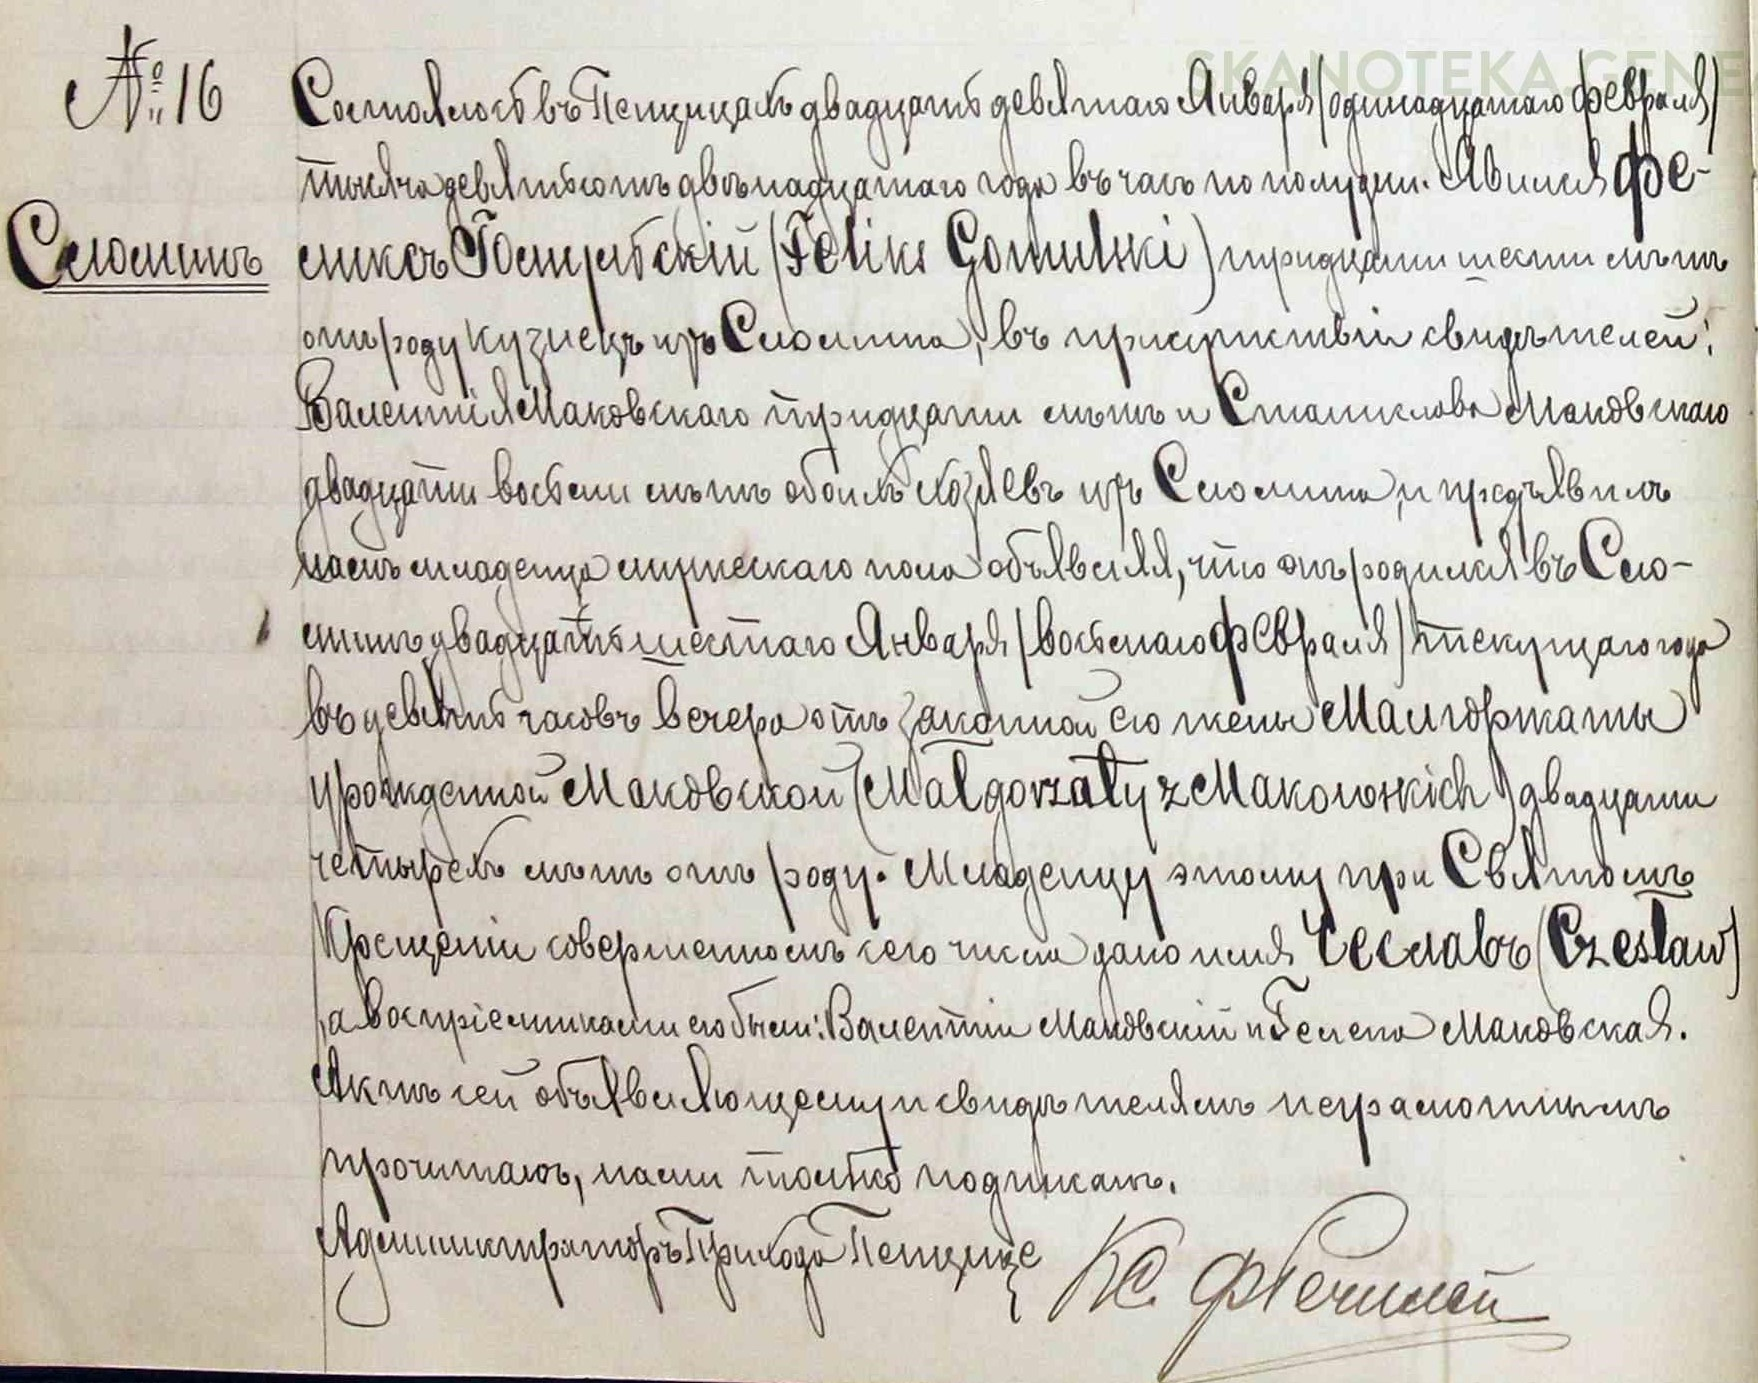
\includegraphics[width=0.8\linewidth]{
        1912_Czesław_Gomulski_akt_chrztu_parafia_Pęcice_wpis_16.jpg}
    \captionsetup{format=hang}
    \caption{Akt chrztu Czesława Gomulskiego - par. Pęcice 1912~rok (16/1912) 
    \cite{par_pecice}.}
    \label{fig:czgomulski_1912}
\end{figure}

Feliks Gomulski razem ze swoją małżonką przez pierwsze kilka lat po ślubie 
mieszkali w~rodzinej wsi Małgorzaty - w~Słominie, o~czym świadczy fakt, iż 
ich dwóch pierwszych synów Henryk (patrz: ryc. \ref{fig:hgomulski_1910}) oraz 
Czesław (patrz: ryc. \ref{fig:czgomulski_1912}) urodziło się (odpowiednio 
w~1910 oraz 1912~roku) właśnie w~tej miejscowości. Trzeci syn małżeństwa 
Gomulskich, Walerian (patrz: ryc. \ref{fig:wgomulski_1914}), urodził się 
w~1914~roku w~Mińsku Mazowieckim, a~ich pierwsza córka, Helena, urodziła 
się (patrz: ryc. \ref{fig:hgomulska_1917}) oraz zmarła (patrz: ryc. 
\ref{fig:hgomulska_1917_2}) w~1917~roku w~Anielinie. Oznacza to, że po około 
8~latach od ślubu, Feliks Gomulskich powrócił do swojej rodzinnej 
miejscowości.

\begin{figure}[!ht]
    \vspace*{0.5cm}
    \centering \includegraphics[width=0.9\linewidth]{
        1914_Walerian_Gomulski_akt_chrztu_parafia_Mińsk_Mazowiecki_wpis_674.jpg}
    \captionsetup{format=hang}
    \caption{Akt chrztu Waleriana Gomulskiego - par. Mińsk Mazowiecki 
    1914~rok (674/1914) 
    \cite{par_minsk2}.}
    \label{fig:wgomulski_1914}
\end{figure}

\begin{figure}[!ht]
    \vspace*{0.5cm}
    \centering \includegraphics[width=1.0\linewidth]{
        1917_Helena_Gomulska_akt_chrztu_parafia_Mińsk_Mazowiecki_wpis_50.jpg}
    \captionsetup{format=hang}
    \caption{Akt chrztu Heleny Gomulskiej - par. Mińsk Mazowiecki 
    1917~rok (50/1917) 
    \cite{par_minsk2}.}
    \label{fig:hgomulska_1917}
\end{figure}

Czwarty syn małżeństwa Gomulskich, Zygmunt, urodził się również 
w~Anielinie, w~1918~roku (patrz: ryc. \ref{fig:zgomulski_1918}), natomiast 
ich druga córka, Janina, podobnie jak jej starszy brat Walerian, urodziła się 
w~Mińsku Mazowieckim, w~1920~roku (patrz: ryc. \ref{fig:jgomulska_1920}). Co 
ciekawe, w~aktach chrztu Heleny, Zygmunta oraz Janiny, ich ojciec, Feliks 
Gomulski określony został jako kowal, w~dwóch pierwszych wskazano, iż 
zamieszkuje on w~Anielinie natomiast w~trzecim, jako jego miejscowość 
zamieszkania wskazano Grzebowilk. Oznacza to, iż Feliks Gomulski, kontynuował 
rodzinną tradycję i~podobnie jak jego ojciec i~dziadek trudnił się pracą 
kowala w~miejscowościach, w~których zamieszkiwał.

\begin{figure}[!ht]
    \vspace*{0.5cm}
    \centering \includegraphics[width=0.9\linewidth]{
        1918_Zygmunt_Gomulski_akt_chrztu_parafia_Mińsk_Mazowiecki_wpis_196.jpg}
    \captionsetup{format=hang}
    \caption{Akt chrztu Zygmunta Gomulskiego - par. Mińsk Mazowiecki 
    1918~rok (196/1918) 
    \cite{par_minsk2}.}
    \label{fig:zgomulski_1918}
\end{figure}

Autor niniejszej książki nie dysponuje informacjami na temat miejsca narodzin, 
dwóch najmłodszych dzieli Feliksa i Magdaleny Gomulskich - Jadwigi 
i~Mieczysława, gdyż w~momencie pisania niniejszej książki, kościelne akta 
chrztów dostępne do publicznego wglądu, kończyły się, w~zależności od 
parafii, na około 1920~roku\footnote{Większość archidiecezji w~Polsce nie 
udostępnia do publicznego wglądu aktów chrztów młodszych niż 100~lat oraz 
aktów ślubów i~zgonów młodszych niż 80~lat - ze względu na prywatność danych 
osobowych.}. Na podstawie grobów rodziny Gomulskich, znajdujących się na 
cmentarzu parafialnym parafii pod wezwaniem św. Kazimierza w~Pruszkowie, 
można jedynie stwierdzić, iż urodzili się oni odpowiednio w~1923 (patrz: ryc. 
\ref{fig:mgomulska_1951}) oraz w~1929~roku (patrz: ryc. 
\ref{fig:czgomulski_1946}).

\begin{figure}[!ht]
    \vspace*{0.5cm}
    \centering \includegraphics[width=0.9\linewidth]{
        1920_Janina_Gomulska_akt_chrztu_parafia_Mińsk_Mazowiecki_wpis_347.jpg}
    \captionsetup{format=hang}
    \caption{Akt chrztu Janiny Gomulskiej - par. Mińsk Mazowiecki 
    1920~rok (347/1920) 
    \cite{par_minsk2}.}
    \label{fig:jgomulska_1920}
\end{figure}

\begin{figure}[!ht]
    \vspace*{0.5cm}
    \centering \includegraphics[width=1.0\linewidth]{
        1917_Helena_Gomulska_akt_zgonu_parafia_Mińsk_Mazowiecki_wpis_303.jpg}
    \captionsetup{format=hang}
    \caption{Akt zgonu Heleny Gomulskiej - par. Mińsk Mazowiecki 
    1917~rok (303/1917) 
    \cite{par_minsk2}.}
    \label{fig:hgomulska_1917_2}
\end{figure}

Feliks i~Małgorzata Gomulscy, jak można wywnioskować na podstawie aktów 
chrztów ich dzieci, bardzo często zmieniali miejsca swojego zamieszkania. 
Były to często przeprowadzki na odległości kilkudziesięciu kilometrów, 
z~jednej strony Warszawy na drugą. Wygląda na to, że w~latach 30. XX wieku 
przeprowadzili się ostatecznie razem z~dziećmi do Pruszkowa, gdzie żyli do 
końca swoich dni - jak wynika z~informacji znajdujących się na ich nagrobkach, 
Feliks Gomulski zmarł w~1941~roku (patrz: ryc. \ref{fig:fgomulski_1941}), 
natomiast jego żona Małgorzata z~Makowskich zmarła w~1951~roku (patrz: ryc. 
\ref{fig:mgomulska_1951}).

\begin{figure}[!ht]
    \vspace*{0.4cm}
    \centering 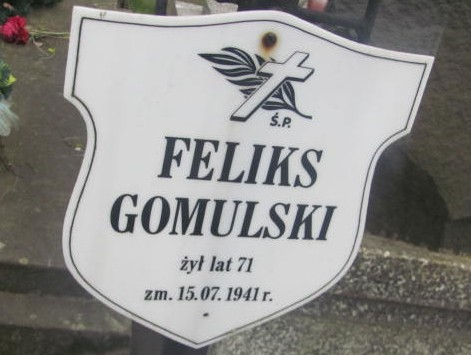
\includegraphics[width=0.6\linewidth]{
        1941_Feliks_Gomulski_zdjęcie_nagrobka1_cmentarz_Pruszków.jpg}
    \captionsetup{format=hang}
    \caption{Zdjęcie tablicy nagrobnej Feliksa Gomulskiego znajdującej się na
    cmentarzu parafialnym parafii pod wezwaniem św. Kazimierza w~Pruszkowie 
    (sektor: P2, rząd: 2, numer: 59)}
    \label{fig:fgomulski_1941}
\end{figure}

Dalsze losy dzieci Feliksa i~Małgorzaty Gomulskich nie są znane autorowi 
niniejszej książki. Jedyne informacje jakie udało się zdobyć, to te 
pochodzące z~nagrobków znajdujących się na parafialnym parafii pod wezwaniem
św. Kazimierza w~Pruszkowie.  Wskazują one, iż Zygmunt Gomulski zmarł
w~1943~roku (patrz: ryc. \ref{fig:zgomulski_1943}), Czesław Gomulski zmarł
w~1946~roku (patrz: ryc.\ref{fig:czgomulski_1946}), Mieczysław Gomulski zmarł
w~1968~roku (patrz: ryc. \ref{fig:czgomulski_1946}), Jadwiga Gomulska zmarła
w~1994~roku (patrz: ryc. \ref{fig:mgomulska_1951}), Walerian Gomulski zmarł
w~1995~roku (patrz: ryc. \ref{fig:mgomulska_1951}), a~Janina Gomulska dożyła
do 2008~roku (patrz: ryc. \ref{fig:zgomulski_1943}).

\begin{figure}[!ht]
    \vspace*{0.4cm}
    \centering 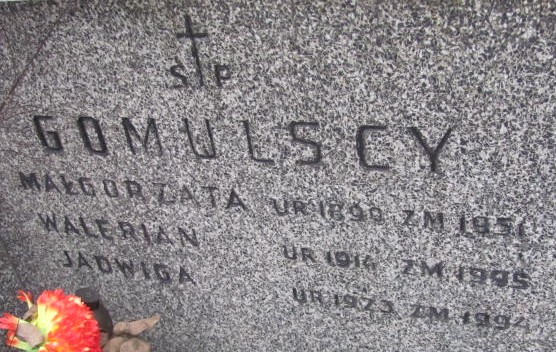
\includegraphics[width=0.7\linewidth]{
        1951_Małgorzata_Gomulska_Makowska_zdjęcie_nagrobka2_cmentarz_Pruszków.jpg}
    \captionsetup{format=hang}
    \caption{Zdjęcie grobu Małgorzaty, Waleriana i~Jadwigi Gomulskich 
    znajdującego się na cmentarzu parafialnym parafii pod wezwaniem św. 
    Kazimierza w~Pruszkowie (sektor: P4, rząd: 3, numer: 21)}
    \label{fig:mgomulska_1951}
\end{figure}

\begin{figure}[!ht]
    \vspace*{0.5cm}
    \centering 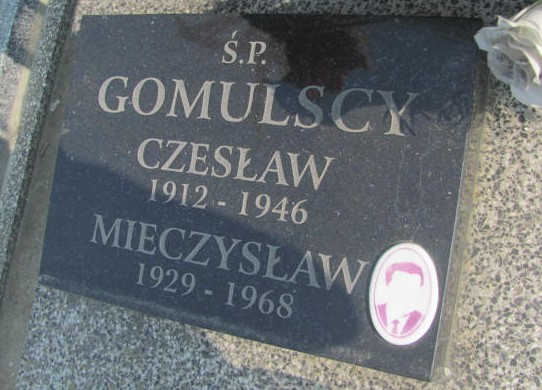
\includegraphics[width=0.87\linewidth]{
        1946_Czesław_Gomulski_zdjęcie_nagrobka1_cmentarz_Pruszków.jpg}
    \captionsetup{format=hang}
    \caption{Zdjęcie grobu Czesława i~Mieczysława Gomulskich znajdującego się 
    na cmentarzu parafialnym parafii pod wezwaniem św. Kazimierza 
    w~Pruszkowie (sektor: B3, rząd: 4, numer: 10)}
    \label{fig:czgomulski_1946}
\end{figure}

\begin{figure}[!ht]
    \vspace*{0.5cm}
    \centering 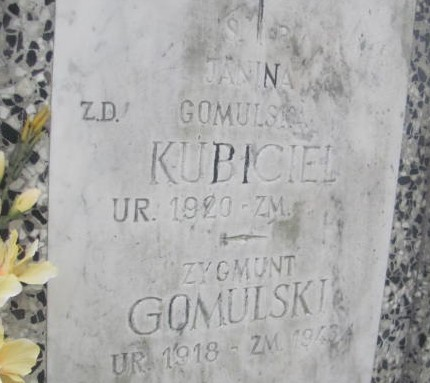
\includegraphics[width=0.6\linewidth]{
        1943_Zygmunt_Gomulski_zdjęcie_nagrobka2_cmentarz_Pruszków.jpg}
    \captionsetup{format=hang}
    \caption{Zdjęcie grobu Zygmunta Gomulskiego i~Janiny Kubiciel 
    znajdującego się na cmentarzu parafialnym parafii pod wezwaniem św. 
    Kazimierza w~Pruszkowie (sektor: P2, rząd: 6, numer: 37)}
    \label{fig:zgomulski_1943}
\end{figure}

Co ciekawe, na stronie Muzeum Powstania Warszawskiego 
(\url{https://www.1944.pl}), widnieje informacja, iż Walerian Gomulski był 
uczestnikiem Powstania Warszawskiego, gdzie walczył w~stopniu strzelca, po 
czym trafił do niemieckiej niewoli - numer jeniecki: 45706 - patrz 
\ref{fig:wgomulski_biogram}\footnote{Biogram Powstańczy:
\url{https://www.1944.pl/powstancze-biogramy/walerian-gomulski,14633.html}}.

\begin{figure}[!ht]
    \vspace*{0.5cm}
    \centering \includegraphics[width=1.0\linewidth]{
        Walerian_Gomulski_biogram_powstańczy.png}
    \captionsetup{format=hang}
    \caption{Biogram Powstańczy Waleriana Gomulskiego ze strony internetowej
    Muzeum Powstania Warszawskiego.}
    \label{fig:wgomulski_biogram}
\end{figure}

Historia rodziny Gomulskich w~Anielinie zakończyłaby się w~latach 30.~XX~wieku,
kiedy to Feliks Gomulski wraz z~rodziną ostatecznie wyprowadził się 
z~tej miejscowości (przenosząc się prawdopodobnie do Pruszkowa), gdyby nie 
fakt, iż około 1921~roku do Anieliny z~Desna przeprowadził się Władysław 
Gomulski (ur. 1901~r. - zm. 1967~r.) najmłodszy syn Stanisława Gomulskiego 
(ur. 1863~r. - zm. 1929~r.), najmłodszego syna Piotra Franciszka Gumulskiego.
Władysław Gomulski wrócił do miejscowości narodzin swojego ojca, gdyż
w~1921~roku ożenił się w~Mińsku Mazowieckim z~Marianną Paszkowską, która 
urodziła się i~wychowała w~Anielinie. Władysław i~Marianna Gomulscy dochowali 
się prawdopodobnie czwórki dzieci: Jerzego (ur.~1922~r. - zm. 1996~r.),
Krystyny (ur. 1924~r. - zm. 2007~r.), Szczepana (ur. 1927~r. - zm. 2014~r.)
oraz Benedykta (ur. 1938~r. - zm. 2021~r.) - wszystkie z~nich urodziły się 
w~Anielinie, a~ich potomkowie mieszkają tam prawdopodobnie do dnia
dzisiejszego\footnote{Oczywiście już nie w~Anielinie, bo od 1~stycznia
1986~roku Anielina stała się częścią Mińska Mazowieckiego i~jedyny widoczny
ślad po tej miejscowości stanowi przystanek kolejowy Mińsk Mazowiecki 
Anielina.}.

% Przednia okładka podrozdziału
\includepdf{Wolka_Minska_mapa_fin.png}

\section{Wólka Mińska: 1861~r. - 2025~r.}

Wólka Mińska została założona, jako wieś szlachecka, w~połowie XVI~wieku 
w~odległości około trzech kilometrów na północ od Mińska Mazowieckiego,
na terenie ziemii czerskiej województwa mazowieckiego. Od początku swojego 
istnienia wieś ta należała do parafii pod wezwaniem Narodzenia Najświętszej 
Maryi Panny w~Mińsku Mazowieckim. Na początku XIX wieku Wólka Mińska 
znajdowała się na terenie zaboru austriackiego, następnie w~1809~roku została 
włączona do Księstwa Warszawskiego, a~w~1815~roku do Królestwa Polskiego. 
Słownik geograficzny Królestwa Polskiego podaje, iż w~1827~roku w~Wólce 
Mińskiej znajdowały się trzy domy, w~których mieszkało 25~osób. Nieopodal 
Wólki Mińskiej swoje źródła ma rzeka Długa\footnote{Rzeka Długa przepływa
również niedaleko wsi Desno, co więcej odegrała ona prawdopodobnie 
istotną rolę w~zdefiniowaniu nazwy tej miejscowości, o~czym szerzej opowiemy 
w~dalszej części niniejszej książki.}.

\begin{figure}[!ht]
    \vspace*{0.5cm}
    \centering 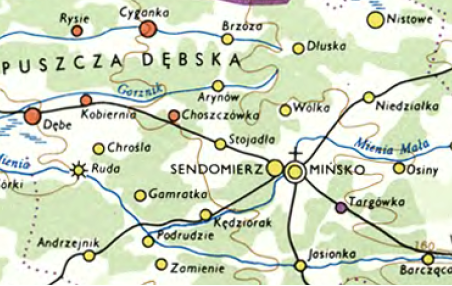
\includegraphics[width=1.0\linewidth]{
        Wólka Mińska - Mazowsze w drugiej połowie XVI wieku.png}
    \captionsetup{format=hang}
    \caption{Mapa miejscowości znajdujących się w~okolicy Mińska Mazowieckiego 
    w~połowie XVI~wieku opracowana w~1972~roku przez Instytut Historii 
    Polskiej Akademii Nauk \cite{palucki}.}
    \label{fig:wolka_minska_xvi}
\end{figure}

Jan Gomulski (ur.~1836~r. - zm.~1901~r.), najstarszy syn Piotra i~Marianny 
Gumulskich, 31~stycznia~1858~roku wziął ślub z~Agnieszką Piotrkowicz 
(ur.~1840~r. - zm.~1881~r.) - patrz: ryc. \ref{fig:jgomulski_1858}. Agnieszka
Piotrkowicz urodziła się 26~grudnia~1840~roku w~Budach Barcząckich (patrz:
ryc. \ref{fig:agumulska_1840}), a~jej rodzice Tomasz oraz Agnieszka (z~domu 
Liszowska) pochodzili z~Dębego Wielkiego\footnote{Historia rodziny
Piotrkowiczów z~Dębego zostanie szerzej omówiona w~\hyperref[sec:piotrkowicze]{
załączniku numer~IV} do niniejszej książki, ze względu na liczne powiązania
członków rodziny Piotrkowiczów z~rodziną Gomulskich.}.

\begin{figure}[!ht]
    \vspace*{0.5cm}
    \centering \includegraphics[width=0.95\linewidth]{
        1840_Agnieszka_Gumulska_Piotrkowicz_akt_chrztu_parafia_Mińsk_Mazowiecki_wpis_314.jpg}
    \captionsetup{format=hang}
    \caption{Akt chrztu Agnieszki Piotrkowicz - par. Mińsk Mazowiecki 
    1840~rok (314/1840) 
    \cite{par_minsk2}.}
    \label{fig:agumulska_1840}
\end{figure}

Przez pierwsze lata po ślubie Jan i~Agnieszka Gomulscy zamieszkiwali jeszcze
w~rodzinnej wsi Jana - w~Anielinie, gdzie 22~stycznia 1859~roku urodził się
ich pierwszy syn Józef (patrz: ryc. \ref{fig:jgomulski_1859}). W~akcie chrztu
Józefa, jego ojciec Jan określony został jako wyrobnik. W~okolicach 1861~roku
Jan i~Agnieszka Gomulscy wraz z~synem Józefem przeprowadzili się do Wólki 
Mińskiej, gdzie 22~lutego 1861~roku urodził się ich drugi syn - Stanisław. 
Rodzicami chrzestnymi Stanisława zostali Kacper Bronikowski oraz Marianna
Frelak, a~jego ojciec w~akcie chrztu został określony jako \enquote{...
gospodarz, ojciec dziecięcia lat dwadzieścia pięć mający w~Wólce
zamieszkały...} (patrz: ryc. \ref{fig:sgomulski_1861}). Stanisław Gomulski był
ostatnim z~trzech członków rodziny Gomulskich, którzy byli współzałożycielami
wsi Desna (a~zarazem udziałowcami spółki \enquote{Desna}) - razem ze swoimi
stryjkami (a~jednocześnie rówieśnikami) Michałem i~Stanisławem (stryj Michał
był od niego o~dwa lata starszy, a~jego stryjk-imiennik o~dwa lata młodszy)
przeprowdził się do wsi Desna w~okoliach 1896~roku. Bezpośredni potomkowie
Stanisława Gomulskiego mieszkają we wsi Desno do dnia dzisiejszego, nosząc
nazwisko po swoim przodku\footnote{Autor niniejszej książki jest
praprawnukiem Stanisława Gomulskiego, mieszka we wsi Desno, a~ponadto urodził
się dokładnie 129~lat po nim – 22 lutego 1990 roku.}.

\begin{figure}[!ht]
    \vspace*{0.5cm}
    \centering 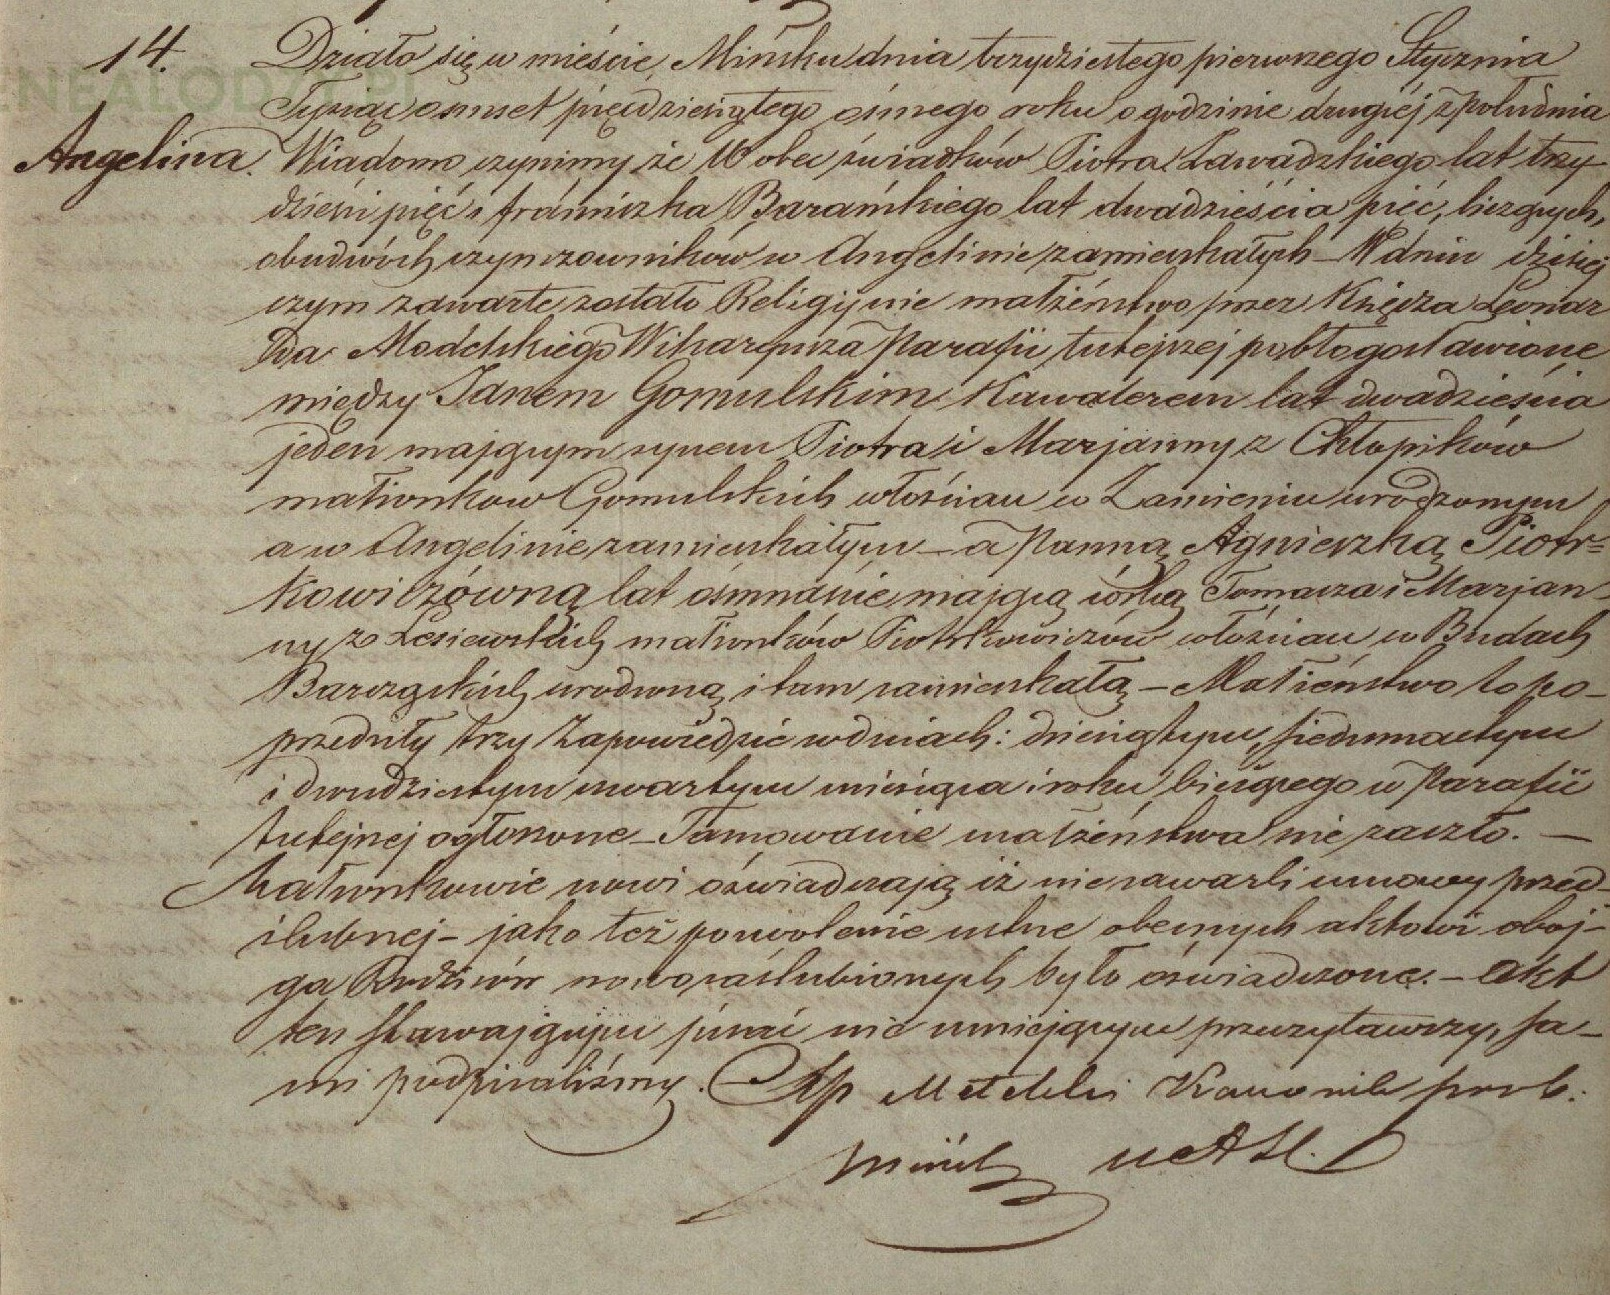
\includegraphics[width=0.92\linewidth]{
        1858_Jan_Gomulski_Agnieszka_Piotrkowicz_akt_ślubu_parafia_Mińsk_Mazowiecki_wpis_14.jpg}
    \captionsetup{format=hang}
    \caption{Akt ślubu Jana Gomulskiego i~Agnieszki Piotrkowicz - par. 
    Mińsk Mazowiecki 1858~rok (14/1858) \cite{par_minsk2}.}
    \label{fig:jgomulski_1858}
\end{figure}

\begin{figure}[!ht]
    \vspace*{0.5cm}
    \centering 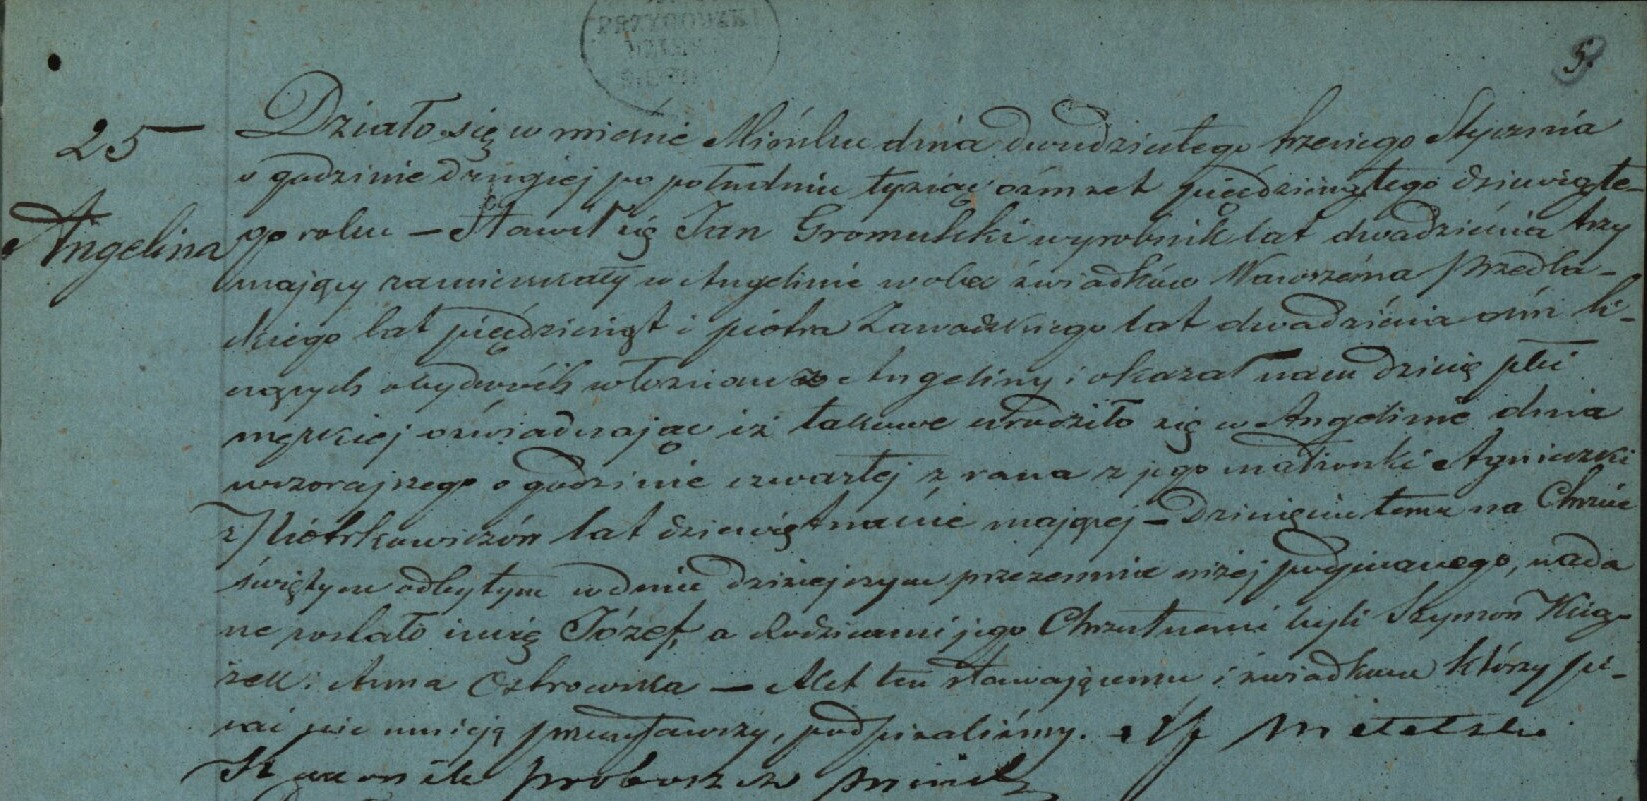
\includegraphics[width=1.0\linewidth]{
        1859_Józef_Gomulski_akt_chrztu_parafia_Mińsk_Mazowiecki_wpis_25.jpg}
    \captionsetup{format=hang}
    \caption{Akt chrztu Józefa Gomulskiego - par. Mińsk Mazowiecki 
    1859~rok (25/1859) 
    \cite{par_minsk2}.}
    \label{fig:jgomulski_1859}
\end{figure}

\begin{figure}[!ht]
    \vspace*{0.5cm}
    \centering 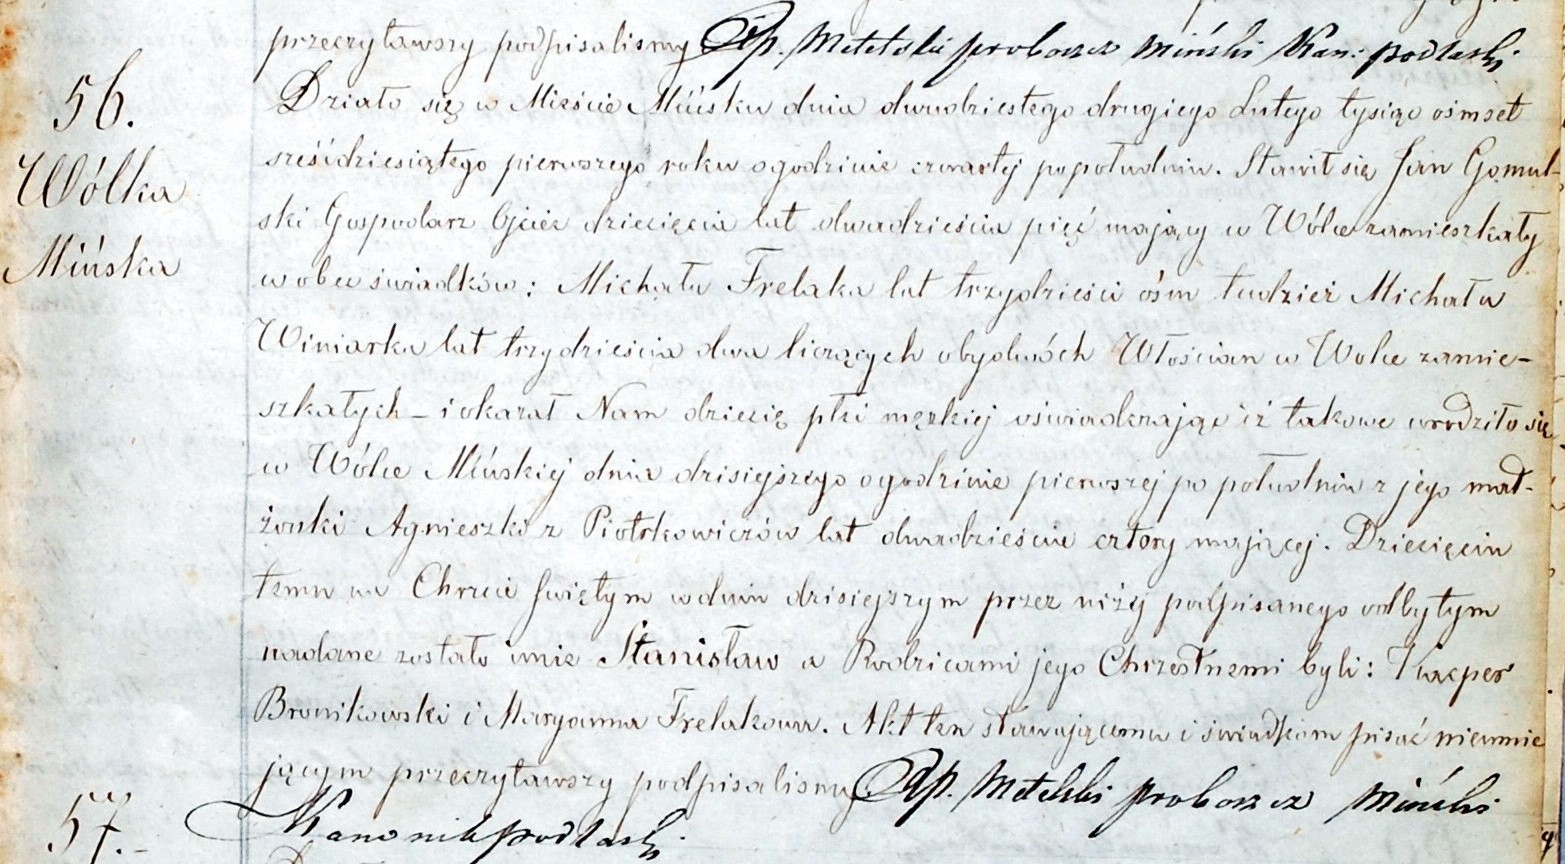
\includegraphics[width=1.0\linewidth]{
        1861_Stanisław_Gomulski_akt_chrztu_parafia_Mińsk_Mazowiecki_wpis_56.jpg}
    \captionsetup{format=hang}
    \caption{Akt chrztu Stanisława Gomulskiego - par. Mińsk Mazowiecki 
    1861~rok (56/1861) 
    \cite{par_minsk2}.}
    \label{fig:sgomulski_1861}
\end{figure}

Jan i~Agnieszka Gomulscy przez 23~lata małżeństwa doczekali się łącznie
dwanaściorga dzieci (wszystkie ich dzieci, poza Józefem, urodziły się w~Wólce
Mińskiej):

\begin{itemize}
    \item Józef Gomulski (ur. 1859~r. - zm. 1929~r.) - patrz: ryc. 
    \ref{fig:jgomulski_1859},
    \item Stanisław Gomulski (ur. 1861~r. - zm. 1910~r.) - patrz: ryc. 
    \ref{fig:sgomulski_1861},
    \item Jan Gomulski (ur. 1863~r. - zm. 1932~r.) - patrz: ryc. 
    \ref{fig:jgomulski_1863},
    \item Julianna Gomulska (ur. 1865~r. - zm. 1868~r.) - patrz: ryc. 
    \ref{fig:jgomulska_1865},
    \item Marianna Gomulska (ur. 1867~r. - zm. 1868~r.) - patrz: ryc. 
    \ref{fig:mgomulska_1867},
    \item Józefa Gomulska (ur. 1869~r. - zm. 1872~r.) - patrz: ryc. 
    \ref{fig:jgomulska_1869},
    \item Anna Gomulska (ur. 1872~r. - zm. ?) - patrz: ryc. 
    \ref{fig:agomulska_1872},
    \item Antonina Paulina Gomulska (ur. 1874~r. - zm. 1877~r.) - patrz: ryc. 
    \ref{fig:apgomulska_1874},
    \item Zofia Gomulska (ur. 1876~r. - zm. 1948~r.) - patrz: ryc. 
    \ref{fig:zgomulska_1876},
    \item Franciszek Gomulski (ur. 1879~r. - zm. 1886~r.) - patrz: ryc. 
    \ref{fig:fgomulski_1879},
    \item Antoni Gomulski (ur. 1879~r. - zm. ?) - patrz: ryc. 
    \ref{fig:agomulski_1879},
    \item Marianna Gomulska (ur. 1881~r. - zm. 1881~r.) - patrz: ryc. 
    \ref{fig:mgomulska_1881}.
  \end{itemize}

Tylko szóstka dzieci małżeństwa Gomulskich dożyła wieku dorosłego: Józef,
Stanisław, Jan, Anna, Zofia oraz Antoni.

\begin{figure}[!ht]
    \vspace*{0.5cm}
    \centering \includegraphics[width=0.9\linewidth]{
        1863_Jan_Gomulski_akt_chrztu_parafia_Mińsk_Mazowiecki_wpis_140.jpg}
    \captionsetup{format=hang}
    \caption{Akt chrztu Jana Gomulskiego - par. Mińsk Mazowiecki 1863~rok (140/1863) 
    \cite{par_minsk2}.}
    \label{fig:jgomulski_1863}
\end{figure}

\begin{figure}[!ht]
    \vspace*{0.5cm}
    \centering \includegraphics[width=0.95\linewidth]{
        1865_Julianna_Gomulska_akt_chrztu_parafia_Mińsk_Mazowiecki_wpis_81.jpg}
    \captionsetup{format=hang}
    \caption{Akt chrztu Julianny Gomulskiej - par. Mińsk Mazowiecki 1865~rok (81/1865) 
    \cite{par_minsk2}.}
    \label{fig:jgomulska_1865}
\end{figure}

\begin{figure}[!ht]
    \vspace*{0.5cm}
    \centering \includegraphics[width=0.95\linewidth]{
        1867_Marianna_Gomulska_akt_chrztu_parafia_Mińsk_Mazowiecki_wpis_60.jpg}
    \captionsetup{format=hang}
    \caption{Akt chrztu Marianny Gomulskiej - par. Mińsk Mazowiecki 1867~rok (60/1867) 
    \cite{par_minsk2}.}
    \label{fig:mgomulska_1867}
\end{figure}

\begin{figure}[!ht]
    \vspace*{0.5cm}
    \centering 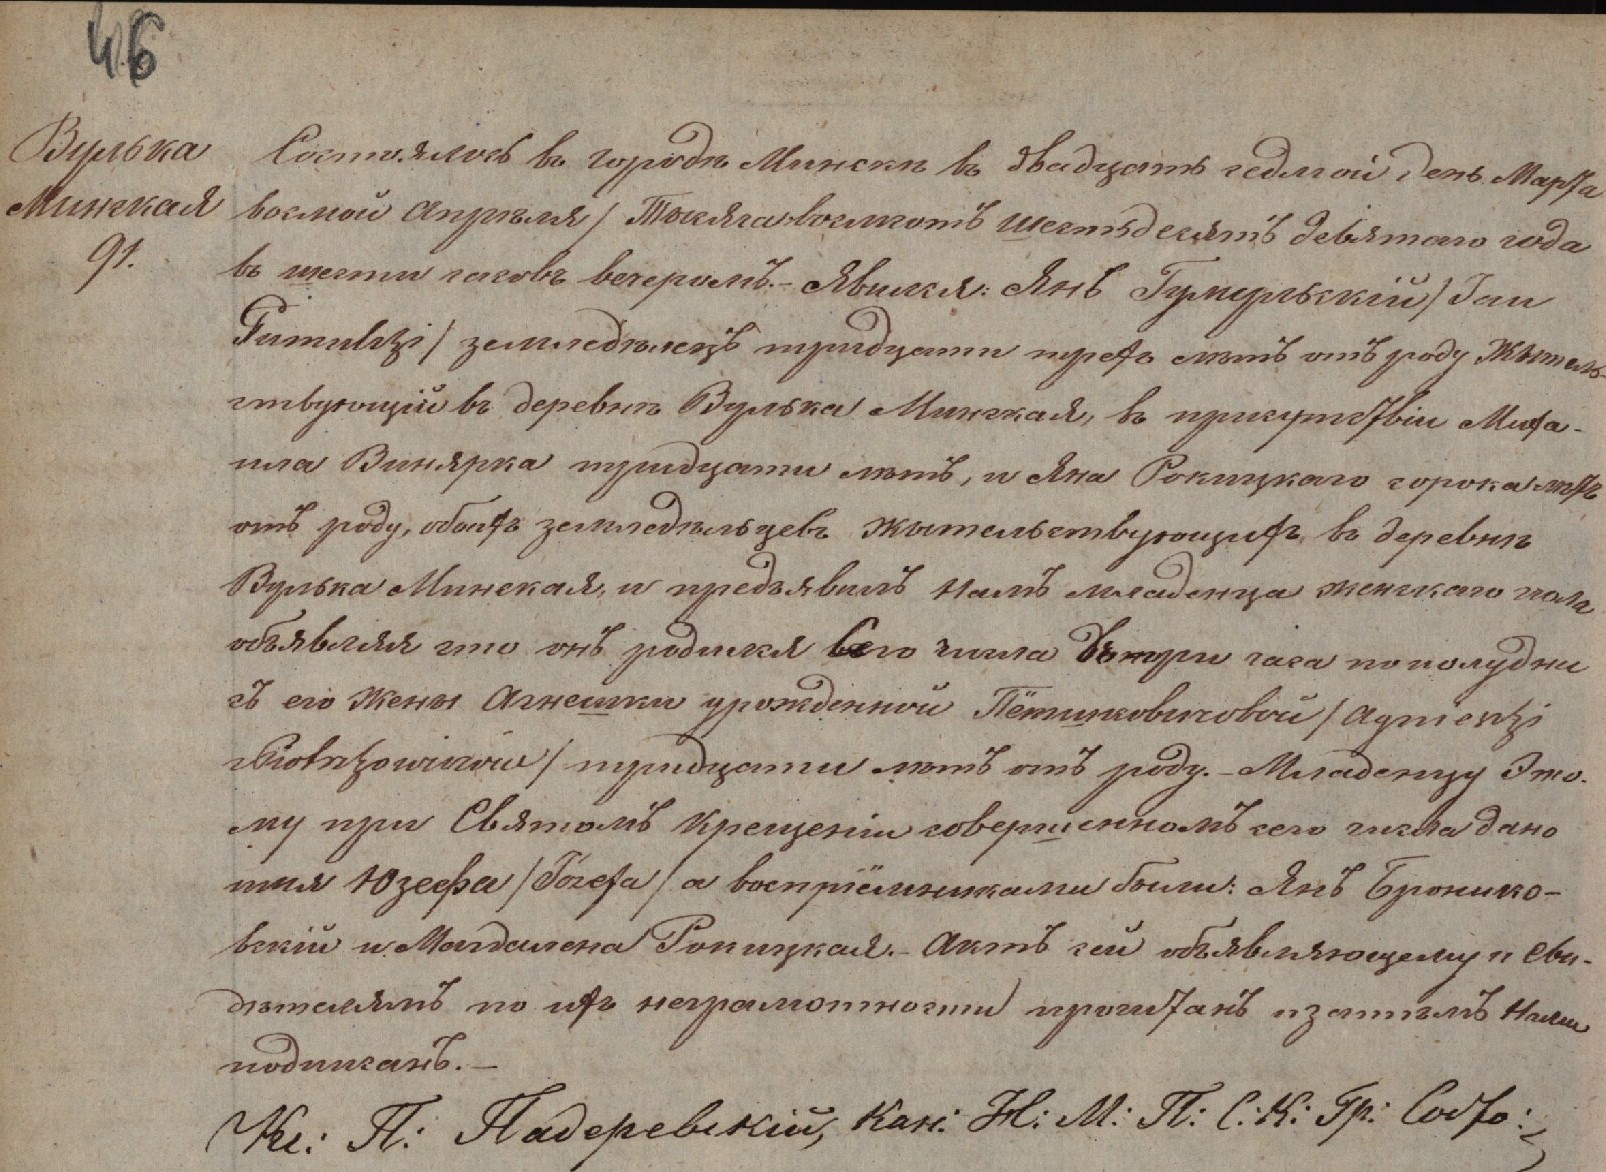
\includegraphics[width=0.95\linewidth]{
        1869_Józefa_Gomulska_akt_chrztu_parafia_Mińsk_Mazowiecki_wpis_91.jpg}
    \captionsetup{format=hang}
    \caption{Akt chrztu Józefy Gomulskiej - par. Mińsk Mazowiecki 1869~rok (91/1869) 
    \cite{par_minsk2}.}
    \label{fig:jgomulska_1869}
\end{figure}

\begin{figure}[!ht]
    \vspace*{0.5cm}
    \centering \includegraphics[width=0.77\linewidth]{
        1872_Anna_Gomulska_Kwiatkowska_akt_chrztu_parafia_Mińsk_Mazowiecki_wpis_98.jpg}
    \captionsetup{format=hang}
    \caption{Akt chrztu Anny Gomulskiej - par. Mińsk Mazowiecki 1872~rok (98/1872) 
    \cite{par_minsk2}.}
    \label{fig:agomulska_1872}
\end{figure}

\begin{figure}[!ht]
    \vspace*{0.5cm}
    \centering \includegraphics[width=0.77\linewidth]{
        1874_Antonina_Paulina_Gomulska_akt_chrztu_parafia_Mińsk_Mazowiecki_wpis_122.jpg}
    \captionsetup{format=hang}
    \caption{Akt chrztu Antoniny Pauliny Gomulskiej - par. Mińsk Mazowiecki
    1874~rok (122/1874) 
    \cite{par_minsk2}.}
    \label{fig:apgomulska_1874}
\end{figure}

\begin{figure}[!ht]
    \vspace*{0.5cm}
    \centering \includegraphics[width=0.82\linewidth]{
        1876_Zofia_Gomulska_Wojdyga_akt_chrztu_parafia_Mińsk_Mazowiecki_wpis_158.jpg}
    \captionsetup{format=hang}
    \caption{Akt chrztu Zofii Gomulskiej - par. Mińsk Mazowiecki 1876~rok (158/1876) 
    \cite{par_minsk2}.}
    \label{fig:zgomulska_1876}
\end{figure}

\begin{figure}[!ht]
    \vspace*{0.5cm}
    \centering \includegraphics[width=0.82\linewidth]{
        1879_Franciszek_Gomulski_akt_chrztu_parafia_Mińsk_Mazowiecki_wpis_15.jpg}
    \captionsetup{format=hang}
    \caption{Akt chrztu Franciszka Gomulskiego - par. Mińsk Mazowiecki
    1879~rok (15/1879) 
    \cite{par_minsk2}.}
    \label{fig:fgomulski_1879}
\end{figure}

\begin{figure}[!ht]
    \vspace*{0.5cm}
    \centering \includegraphics[width=0.82\linewidth]{
        1879_Antoni_Gomulski_akt_chrztu_parafia_Mińsk_Mazowiecki_wpis_16.jpg}
    \captionsetup{format=hang}
    \caption{Akt chrztu Antoniego Gomulskiego - par. Mińsk Mazowiecki
    1879~rok (16/1879) 
    \cite{par_minsk2}.}
    \label{fig:agomulski_1879}
\end{figure}

\begin{figure}[!ht]
    \vspace*{0.5cm}
    \centering \includegraphics[width=0.82\linewidth]{
        1881_Marianna_Gomulska_akt_chrztu_parafia_Mińsk_Mazowiecki_wpis_124.jpg}
    \captionsetup{format=hang}
    \caption{Akt chrztu Marianny Gomulskiej - par. Mińsk Mazowiecki
    1881~rok (124/1881) 
    \cite{par_minsk2}.}
    \label{fig:mgomulska_1881}
\end{figure}

Agnieszka Gomulska z~domu Piotrkowicz zmarła w~Wólce Mińskiej 27~kwietnia
1881~roku, w~wieku 40~lat (patrz: ryc. \ref{fig:agomulska_1881}). Przyczyną
jej śmierci były prawdopodobnie powikłania po porodowe, gdyż kilka dni
wcześniej, 19~kwietnia 1881~roku, urodziła ona swoją najmłodszą córkę Mariannę,
która również zmarła tego samego dnia co jej matka.

\begin{figure}[!ht]
    \vspace*{0.5cm}
    \centering \includegraphics[width=0.75\linewidth]{
        1881_Agnieszka_Gumulska_Piotrkowicz_akt_zgonu_parafia_Mińsk_Mazowiecki_wpis_105.jpg}
    \captionsetup{format=hang}
    \caption{Akt zgonu Agnieszki Gomulskiej (z~domu Piotrkowicz) - par. Mińsk
    Mazowiecki 1881~rok (105/1881) 
    \cite{par_minsk2}.}
    \label{fig:agomulska_1881}
\end{figure}

Jan Gomulski niecałe dwa miesiące po śmierci swojej żony Agnieszki, 16~czerwca
1881~roku, ożenił się ponownie - z~26~lat młodszą, niespełna dwudziestoletnią,
Wiktorią Świętochowską (ur. 1862~r. - zm. 1937~r.) z~pobliskiej wsi
Dłużka (patrz: ryc. \ref{fig:jgomulski_1881})\footnote{Co ciekawe trzeci syn
Jana z~pierwszego małżeństwa, również Jan, zaledwie pieć miesięcy później
ożenił się z~młodszą siostrą swojej macochy - Marianną Świętochowską (ur.
1864~r. - zm. 1912~r.).}. Jan i~Wiktoria Gomulscy doczekali się razem
jedenaściorga dzieci:

\begin{itemize}
    \item Marianna Gomulska (ur. 1882~r. - zm. 1953~r.) - patrz: ryc. 
    \ref{fig:mgomulska_1882},
    \item Józef Gomulski (ur. 1884~r. - zm. 1929~r.) - patrz: ryc. 
    \ref{fig:jgomulski_1884},
    \item Ludwik Gomulski (ur. 1886~r. - zm. ?) - patrz: ryc. 
    \ref{fig:lgomulski_1886},
    \item Franciszek Stefan Gomulski (ur. 1889~r. - zm. 1889~r.) - patrz: ryc. 
    \ref{fig:fsgomulski_1889},
    \item Bezimienna Gomulska (ur. 1891~r. - zm. 1891~r.) - patrz: ryc. 
    \ref{fig:bgomulska_1891},
    \item Władysław Gomulski (ur. 1892~r. - zm. 1893~r.) - patrz: ryc. 
    \ref{fig:wgomulski_1892},
    \item Eleonora Gomulska (ur. 1894~r. - zm. 1957~r.) - patrz: ryc. 
    \ref{fig:egomulska_1894},
    \item Mieczysław Gomulski (ur. 1896~r. - zm. 1967~r.),
    \item Wanda Gomulska (ur. 1898~r. - zm. 1898~r.),
    \item Bronisław Gomulski (ur. 1899~r. - zm. 1905~r.),
    \item Wanda Gomulska (ur. 1901~r. - zm. 1978~r.).
  \end{itemize}

  \begin{figure}[!ht]
    \vspace*{0.5cm}
    \centering 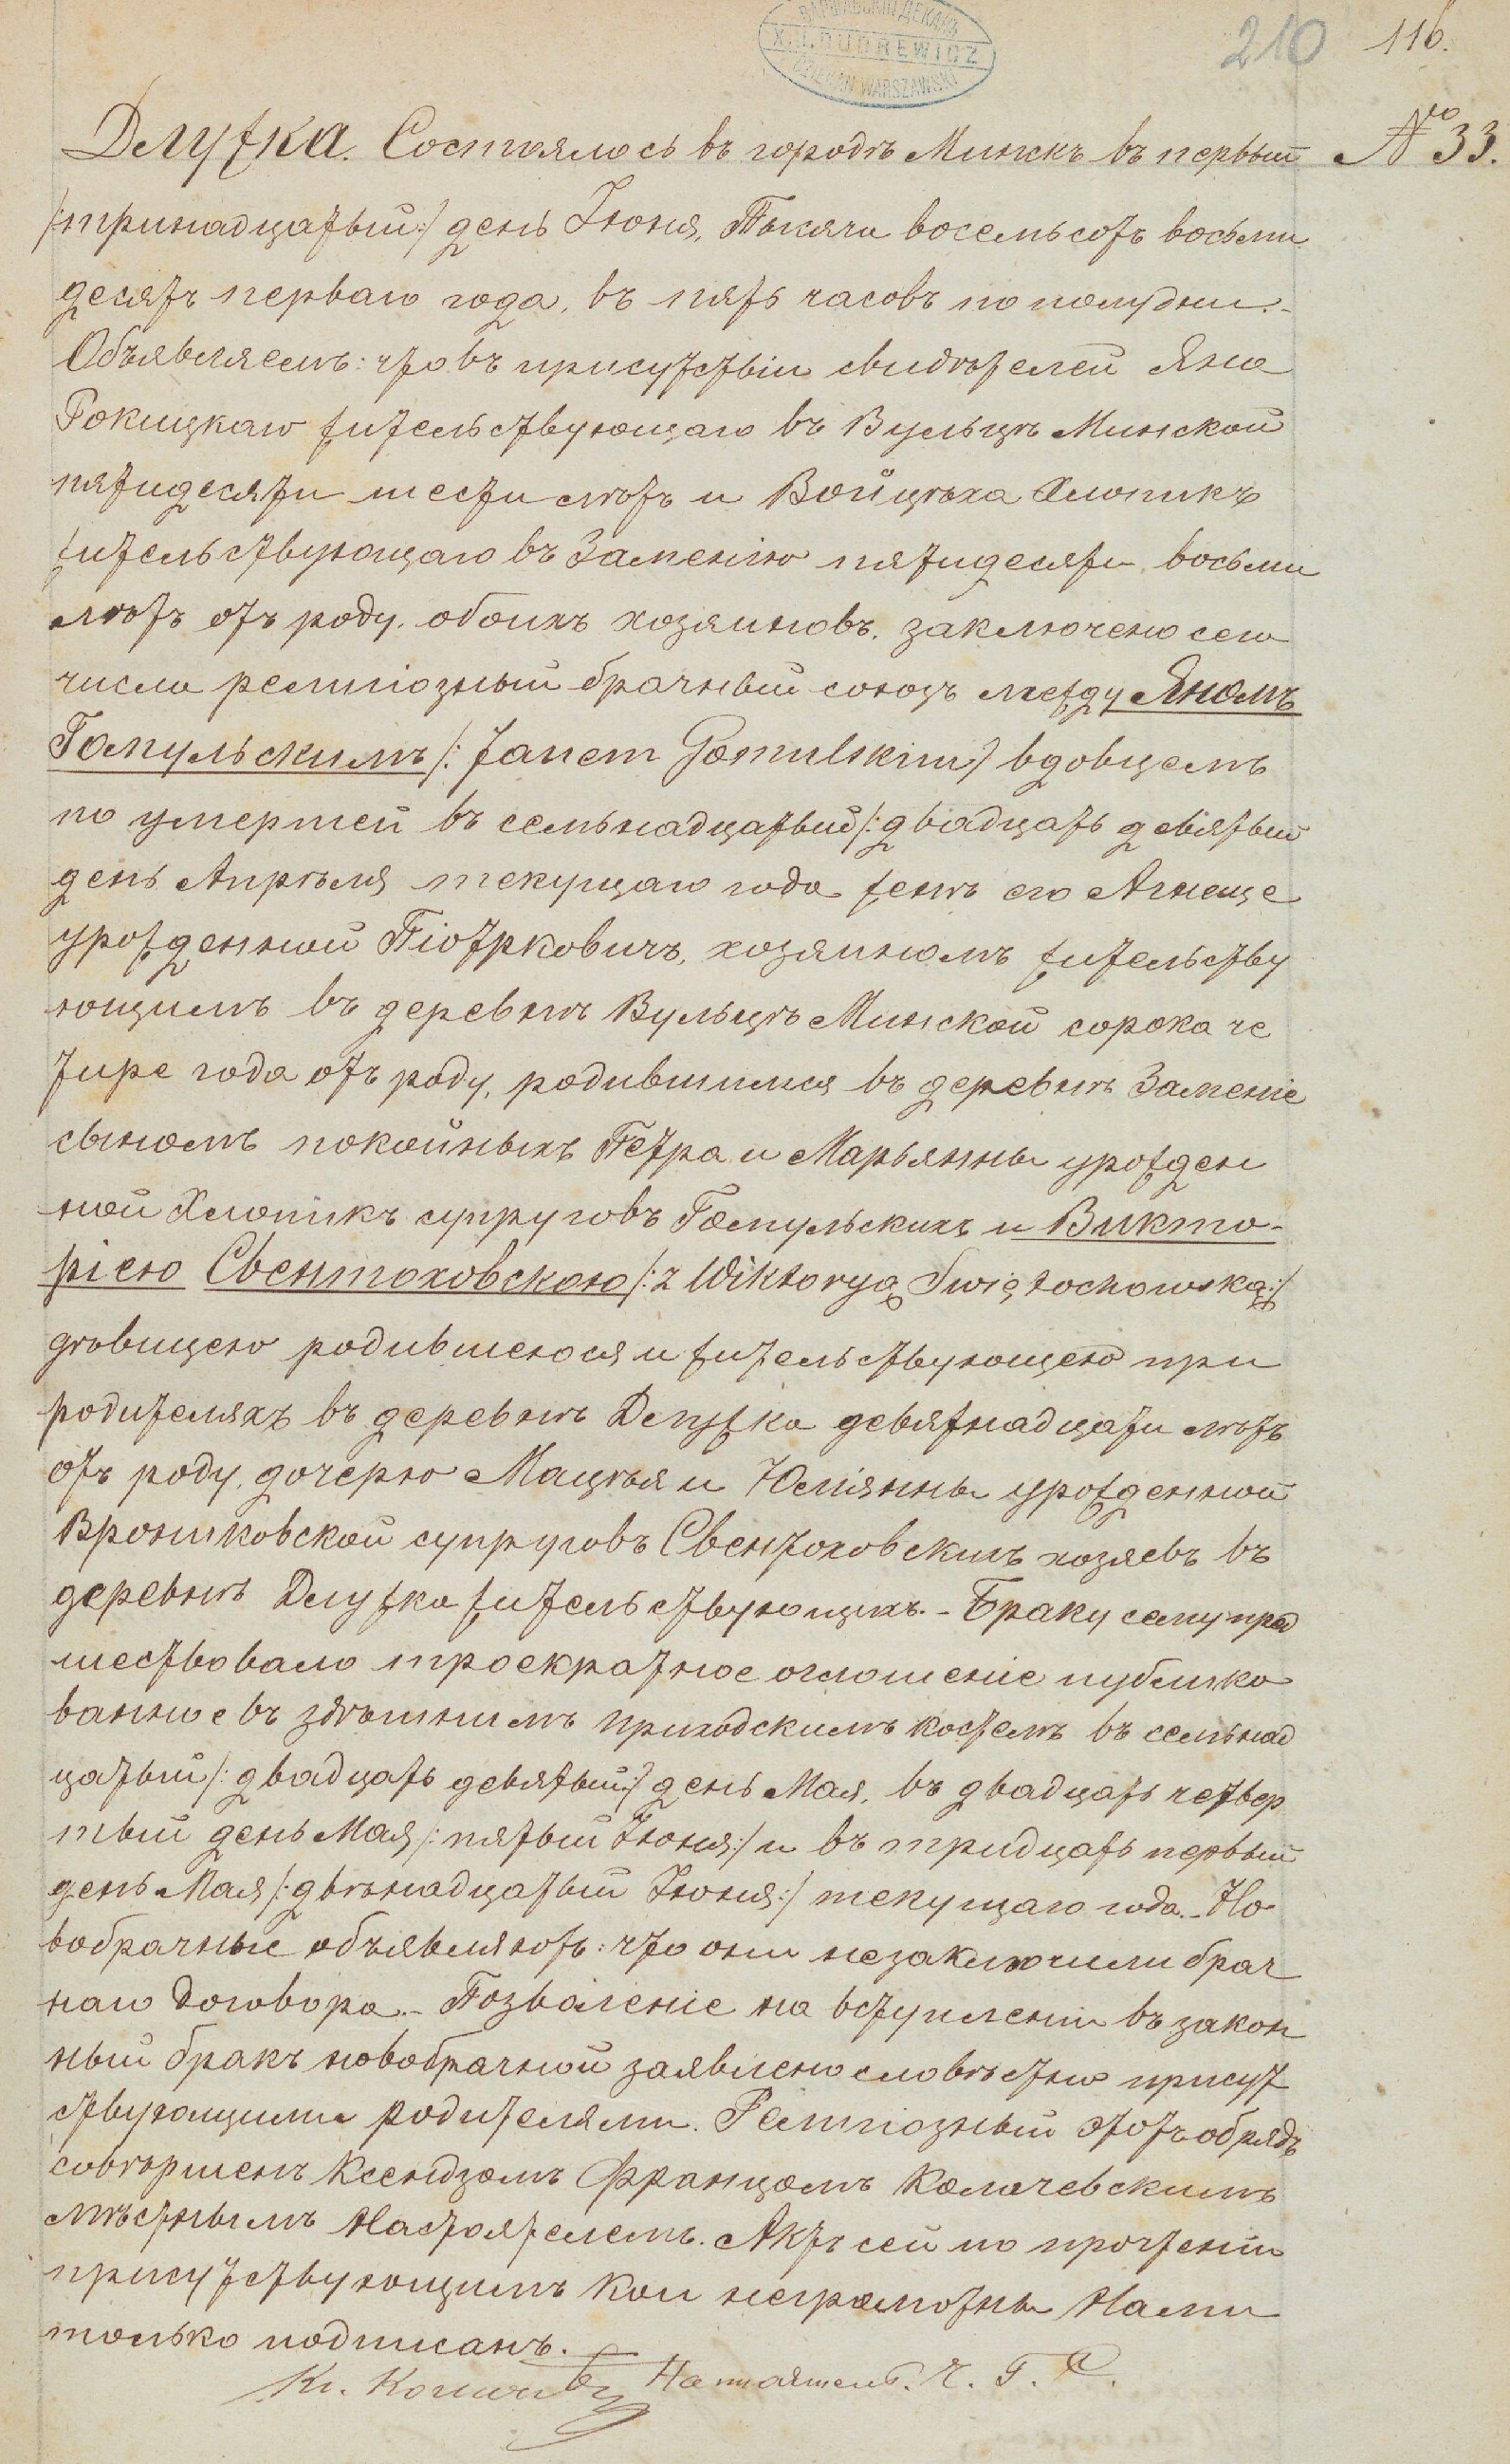
\includegraphics[width=0.85\linewidth]{
        1881_Jan_Gumulski_Wiktoria_Świętochowska_akt_ślubu_parafia_Mińsk_Mazowiecki_wpis_33.jpg}
    \captionsetup{format=hang}
    \caption{Akt ślubu Jana Gomulskiego i~Wiktorii Świętochowskiej - par. 
    Mińsk Mazowiecki 1881~rok (33/1881) \cite{par_minsk2}.}
    \label{fig:jgomulski_1881}
\end{figure}

\begin{figure}[!ht]
    \vspace*{0.5cm}
    \centering 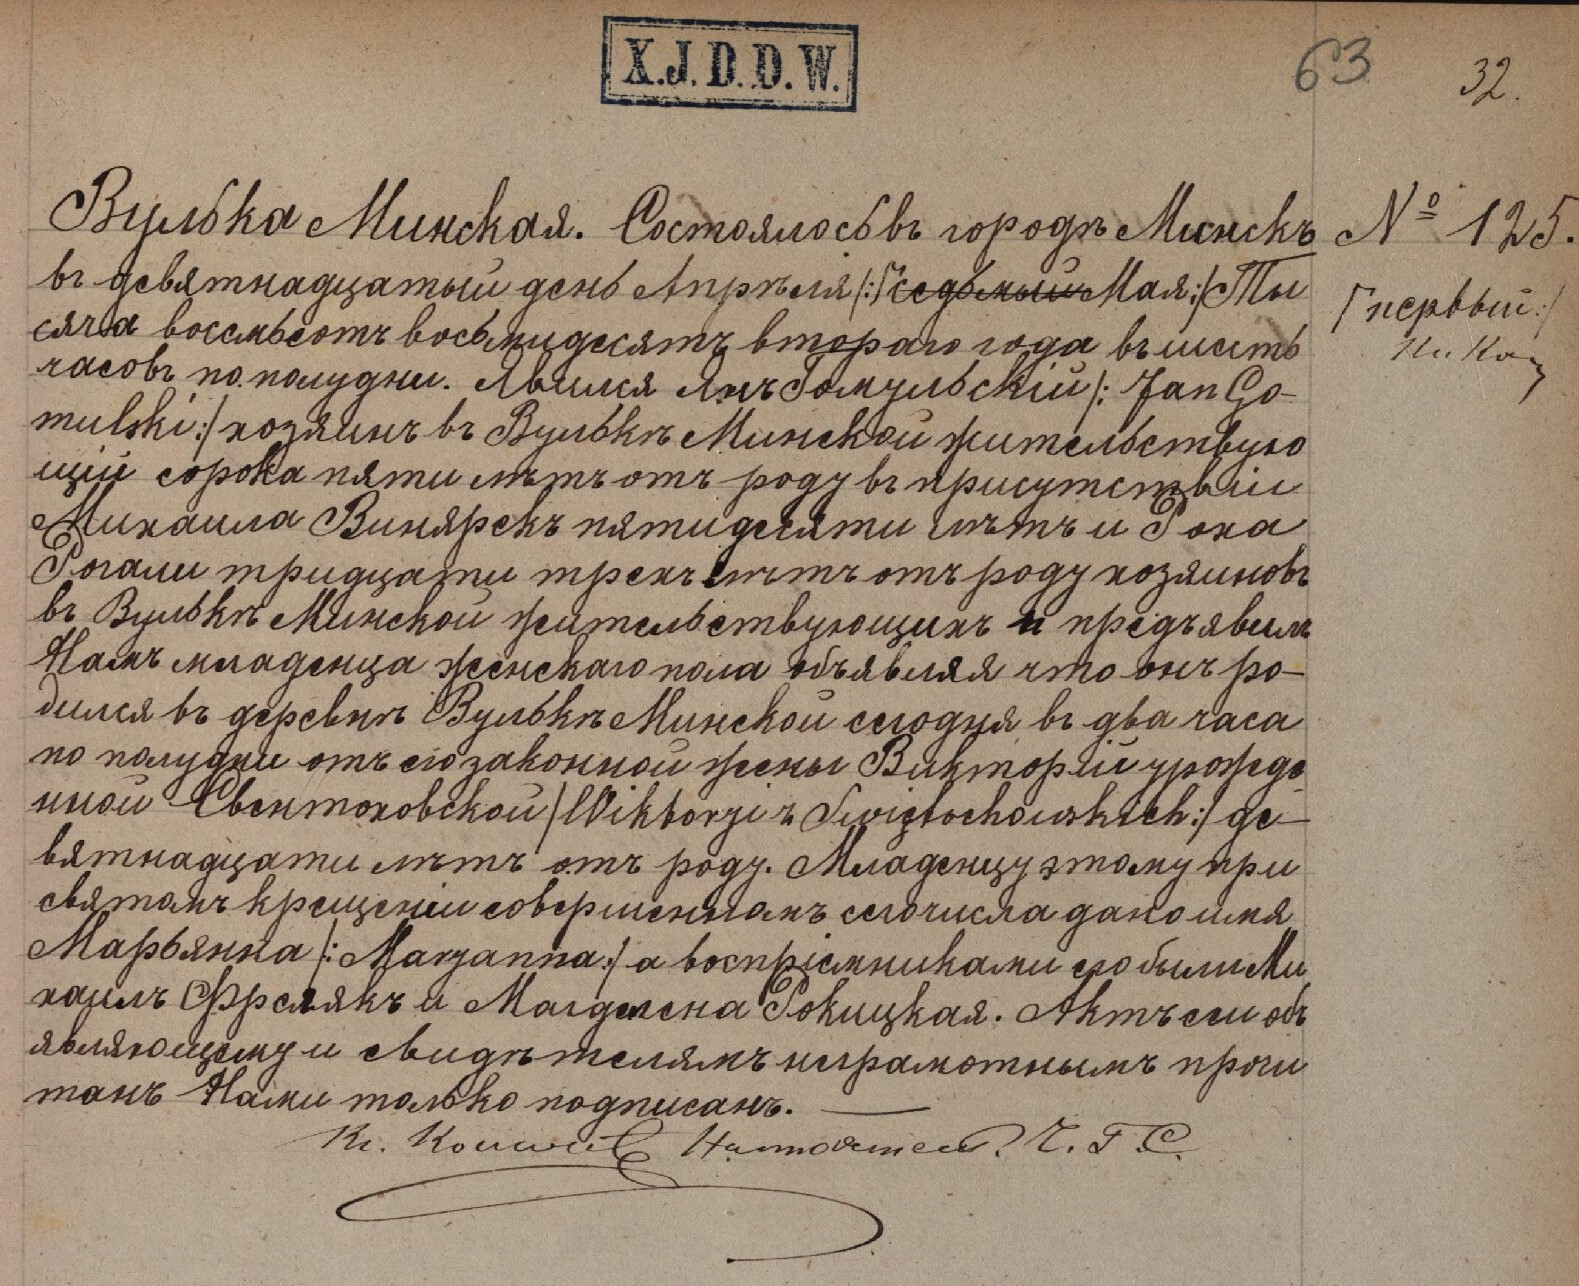
\includegraphics[width=0.77\linewidth]{
        1882_Marianna_Gomulska_Królak_akt_chrztu_parafia_Mińsk_Mazowiecki_wpis_125.jpg}
    \captionsetup{format=hang}
    \caption{Akt chrztu Marianny Gomulskiej - par. Mińsk Mazowiecki
    1892~rok (125/1892) 
    \cite{par_minsk2}.}
    \label{fig:mgomulska_1882}
\end{figure}

\begin{figure}[!ht]
    \vspace*{0.5cm}
    \centering 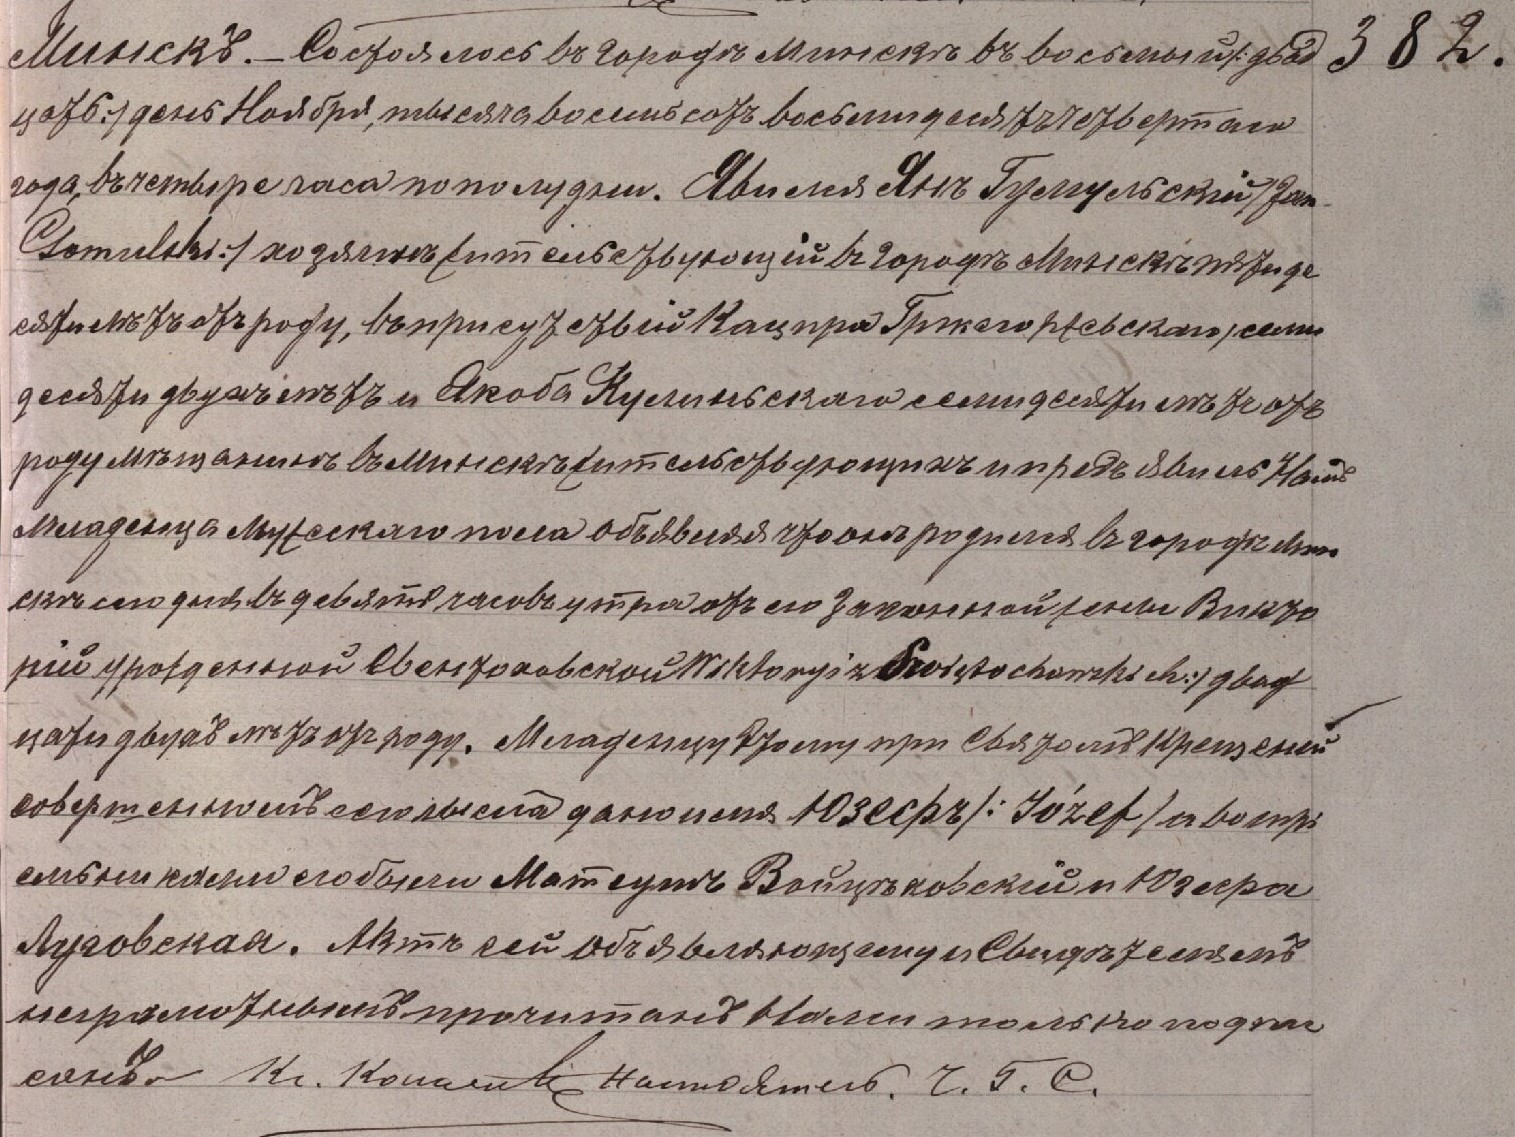
\includegraphics[width=0.77\linewidth]{
        1884_Józef_Gomulski_akt_chrztu_parafia_Mińsk_Mazowiecki_wpis_382.jpg}
    \captionsetup{format=hang}
    \caption{Akt chrztu Józefa Gomulskiego - par. Mińsk Mazowiecki
    1884~rok (382/1884) 
    \cite{par_minsk2}.}
    \label{fig:jgomulski_1884}
\end{figure}

\begin{figure}[!ht]
    \vspace*{0.5cm}
    \centering \includegraphics[width=0.8\linewidth]{
        1886_Ludwik_Gomulski_akt_chrztu_parafia_Mińsk_Mazowiecki_wpis_386.jpg}
    \captionsetup{format=hang}
    \caption{Akt chrztu Ludwika Gomulskiego - par. Mińsk Mazowiecki
    1886~rok (386/1886) 
    \cite{par_minsk2}.}
    \label{fig:lgomulski_1886}
\end{figure}

\begin{figure}[!ht]
    \vspace*{0.5cm}
    \centering \includegraphics[width=0.8\linewidth]{
        1889_Franciszek_Stefan_Gomulski_akt_chrztu_parafia_Mińsk_Mazowiecki_wpis_8.jpg}
    \captionsetup{format=hang}
    \caption{Akt chrztu Franciszka Stefana Gomulskiego - par. Mińsk Mazowiecki
    1889~rok (8/1889) 
    \cite{par_minsk2}.}
    \label{fig:fsgomulski_1889}
\end{figure}

\begin{figure}[!ht]
    \vspace*{0.5cm}
    \centering \includegraphics[width=0.8\linewidth]{
        1891_Bezimienna_Gomulska_akt_chrztu_akt_zgonu_parafia_Mińsk_Mazowiecki_wpis_124.jpg}
    \captionsetup{format=hang}
    \caption{Akt chrztu Bezimiennej Gomulskiej - par. Mińsk Mazowiecki
    1891~rok (124/1891) 
    \cite{par_minsk2}.}
    \label{fig:bgomulska_1891}
\end{figure}

\begin{figure}[!ht]
    \vspace*{0.5cm}
    \centering \includegraphics[width=0.8\linewidth]{
        1892_Władysław_Gomulski_akt_chrztu_parafia_Mińsk_Mazowiecki_wpis_218.jpg}
    \captionsetup{format=hang}
    \caption{Akt chrztu Władysława Gomulskiego - par. Mińsk Mazowiecki
    1892~rok (218/1892) 
    \cite{par_minsk2}.}
    \label{fig:wgomulski_1892}
\end{figure}

\begin{figure}[!ht]
    \vspace*{0.5cm}
    \centering \includegraphics[width=0.82\linewidth]{
        1894_Eleonora_Gomulska_Wilk_akt_chrztu_parafia_Mińsk_Mazowiecki_wpis_460.jpg}
    \captionsetup{format=hang}
    \caption{Akt chrztu Eleonory Gomulskiej - par. Mińsk Mazowiecki
    1894~rok (460/1894)
    \cite{par_minsk2}.}
    \label{fig:egomulska_1894}
\end{figure}

\begin{figure}[!ht]
    \vspace*{0.5cm}
    \centering \includegraphics[width=0.82\linewidth]{
        1937_Wiktoria_Gumulska_Świętochowska_akt_zgonu_parafia_Mińsk_Mazowiecki_wpis_344.jpg}
    \captionsetup{format=hang}
    \caption{Akt zgonu Wiktorii Gomulskiej z d. Świętochowskiej - par. Mińsk Mazowiecki 
    1937~rok (344/1937) \cite{par_minsk2}.}
    \label{fig:wgomulska_1937}
\end{figure}

Jan i~Wiktoria Gomulscy po ślubie zamieszkali w~Wólce Mińskiej, gdzie
urodziła się ich pierwsza córka Marianna, od 1884~roku, przez około 10~lat
mieszkali w~Mińsku Mazowieckim, gdzie na świat przyszli Józef, Ludwik,
Franciszek Stefan, Bezimienna oraz Władysław, po czym wrócili spowrotem do
Wólki Mińskiej, gdzie urodziły się ich kolejne dzieci: Eleonora, Mieczysław,
Bronisław oraz Wanda, oraz gdzie oboje dożyli kresu swoich dni. Jan Gomulski
zmarł 1~marca 1901~roku w~Wólce Mińskiej, w~wieku 65~lat, 5~miesięcy przed
urodzeniem się jego ostatniego dziecka - córki Wandy. Dochował się on łącznie
dwudziestu trojga dzieci z~dwóch małżeństw, z~czego wiemy, iż jedenaścioro
z~nich na pewno dożyło dorosłości. Wiktoria Gomulska zmarła 36~lat po swoimi
mężu, 3~grudnia 1937~roku w~Wólce Mińskiej, w~wieku 75~lat (patrz: ryc. 
\ref{fig:wgomulska_1937}).

\begin{figure}[!ht]
    \vspace*{0.4cm}
    \centering \includegraphics[width=0.95\linewidth]{
        1932_Jan_Gomulski_zdjęcie_nagrobka1_cmentarz_Mińsk_Mazowiecki.jpg}
    \captionsetup{format=hang}
    \caption{Zdjęcie tablicy nagrobnej Jana Gomulskiego znajdującej się na
    cmentarzu parafialnym parafii pod wezwaniem Narodzenia Najświętszej Maryi
    Panny w~Mińsku Mazowieckim (sektor: XIII, rząd: 15, numer: 18)}
    \label{fig:jgomulski_1932}
\end{figure}

Potomkowie Jana Gomulskiego i~jego dwóch żon, mieszkają do dnia dzisiejszego
w~Wólce Mińskiej, w~Mińsku Mazowieckim oraz w~okolicznych miejscowościach:
w~Karolinie, w~Dłużce, w~Arynowie czy w~Targówku. Świadczą o~tym liczne
nagrobki na cmentarzu parafialnym parafii pod wezwaniem Narodzenia
Najświętszej Maryi Panny w~Mińsku Mazowieckim (ul. Kościelna~1, 05-300 Mińsk
Mazowiecki), gdzie spoczywa wielu członków rodziny Gomulskich, zarówno
bezpośrednich potomków Jana Gomulskiego, jak i~potomków jego braci i~sióstr.

\begin{figure}[!ht]
    \vspace*{0.4cm}
    \centering \includegraphics[width=0.75\linewidth]{
        1957_Eleonora_Gomulska_Klimek_Wilk_zdjęcie_nagrobka1_cmentarz_Mińsk_Mazowiecki.jpg}
    \captionsetup{format=hang}
    \caption{Zdjęcie tablicy nagrobnej Wiktorii Gomulskiej 
    z~d.~Świętochowskiej, Eleonory Klimek-Wilk z~d.~Gomulskiej oraz Stanisława
    Klimka znajdującej się na cmentarzu parafialnym parafii pod wezwaniem
    Narodzenia Najświętszej Maryi Panny w~Mińsku Mazowieckim (sektor: XVIII,
    rząd: 5, numer: 32)}
    \label{fig:wgomulska_1957}
\end{figure}

\begin{figure}[!ht]
    \vspace*{0.4cm}
    \centering \includegraphics[width=0.75\linewidth]{
        1948_Zofia_Gomulska_Wojdyga_zdjęcie_nagrobka1_cmentarz_Mińsk_Mazowiecki.jpg}
    \captionsetup{format=hang}
    \caption{Zdjęcie tablicy nagrobnej Zofii Wojdygii z~d.~Gomulskiej
    znajdującej się na cmentarzu parafialnym parafii pod wezwaniem Narodzenia
    Najświętszej Maryi Panny w~Mińsku Mazowieckim (sektor: V, rząd: 14,
    numer: 12)}
    \label{fig:zgomulska_1948}
\end{figure}

\begin{figure}[!ht]
    \vspace*{0.4cm}
    \centering \includegraphics[width=0.8\linewidth]{
        1953_Marianna_Gomulska_Królak_zdjęcie_nagrobka1_cmentarz_Mińsk_Mazowiecki.jpg}
    \captionsetup{format=hang}
    \caption{Zdjęcie tablicy nagrobnej Marianny Królak z~d.~Gomulskiej
    znajdującej się na cmentarzu parafialnym parafii pod wezwaniem Narodzenia
    Najświętszej Maryi Panny w~Mińsku Mazowieckim (sektor: XVI, rząd: 26,
    numer: 14)}
    \label{fig:mgomulska_1953}
\end{figure}

\begin{figure}[!ht]
    \vspace*{0.4cm}
    \centering \includegraphics[width=0.75\linewidth]{
        1957_Mieczysław_Gomulski_zdjęcie_nagrobka1_cmentarz_Mińsk_Mazowiecki.jpg}
    \captionsetup{format=hang}
    \caption{Zdjęcie tablicy nagrobnej Mieczysława i~Marianny Gomulskich
    znajdującej się na cmentarzu parafialnym parafii pod wezwaniem Narodzenia
    Najświętszej Maryi Panny w~Mińsku Mazowieckim (sektor: IX, rząd: 9,
    numer: 14)}
    \label{fig:mgomulski_1957}
\end{figure}

\begin{figure}[!ht]
    \vspace*{0.4cm}
    \centering \includegraphics[width=0.75\linewidth]{
        1957_Wanda_Gomulska_Majszyk_zdjęcie_nagrobka1_cmentarz_Mińsk_Mazowiecki.jpg}
    \captionsetup{format=hang}
    \caption{Zdjęcie tablicy nagrobnej Wandy Majszyk z~d.~Gomulskiej
    znajdującej się na cmentarzu parafialnym parafii pod wezwaniem Narodzenia
    Najświętszej Maryi Panny w~Mińsku Mazowieckim (sektor: XI, rząd: 28,
    numer: 14)}
    \label{fig:wgomulska_1957}
\end{figure}

\begin{figure}[!ht]
    \vspace*{0.4cm}
    \centering \includegraphics[width=0.75\linewidth]{
        1935_Anna_Gomulska_Dobrzyńska_zdjęcie_nagrobka1_cmentarz_Mińsk_Mazowiecki.jpg}
    \captionsetup{format=hang}
    \caption{Zdjęcie tablicy nagrobnej Anny Gomulskiej z~d.~Dobrzyńskiej oraz
    Stanisława Gomulskiego (żony i~syna najstarszego syna Jana Gomulskiego -
    Józefa) znajdującej się na cmentarzu parafialnym parafii pod wezwaniem
    Narodzenia Najświętszej Maryi Panny w~Mińsku Mazowieckim (sektor: XVIII,
    rząd: 1, numer: 6)}
    \label{fig:agomulska_1935}
\end{figure}

Ze wszystkich dzieci Jana Gomulskiego, najdalej od rodzinnej Wólki Mińskiej
wyprowadził się drugi syn Jana z~pierwszego małżeństwa - Stanisław Gomulski,
który w~okolicach 1896~roku stał się jednym ze współzałożycieli (razem ze
swoimi stryjkami Michałem i~Stanisławem), oddalonej o~około 13~kilometrów na
wschód od Wólki Mińskiej, wsi Desna (obecnie Desno).

\newpage
\ifodd\value{page}\hbox{}\newpage\fi

% Przednia okładka podrozdziału
\includepdf{Mikanow_mapa_fin.png}

\section{Mikanów: 1882~r. - 1894~r.}

W~bieżącym


\newpage
\ifodd\value{page}\hbox{}\newpage\fi

% Przednia okładka podrozdziału
\includepdf{Karolina_mapa_fin.png}

\section{Karolina: 1896~r. - 2025~r.}

W~bieżącym
